\chapter{Groups}

\begin{definition}[Closure]
    Let $G$ be a set. A binary operation on $G$ is a function that assigns each ordered pair of elements of $G$ an element of $G$.
    This condition is called \bred{closure}.
\end{definition}

The most familiar binary operations are ordinary addition, subtraction and 
multiplication of integers. However, the division of integers is not a binary operation
on the integers. 

\begin{definition}[Binary operation]
    Let $G$ be a group. A \bred{binary operation} is a map of sets:
    \[
        * : G \times G \to G.
    \]
\end{definition}
For ease of notation we write $*(a,b) = a * b \quad \forall a,b \in G$. Any binary operation on $G$ gives a way of 
combining elements. As we have seen, if $G =\mathbb{Z}$ then $+$ and $\times$ are natural example of binary operations. 

\begin{center}
    {
    \renewcommand{\arraystretch}{2}
    \begin{tabular}{| m{20em} | m{20em} |}
        \hline
        Additive Group & Multiplicative Group\\
        \hline
        Let $G$ be a set, and ${\color{red} +}$ be an operation, 
        then $(G, {\color{red} +})$ is an additive group provided & 
        Let $G$ be a set, and  be an operation, 
        then $(G, {\color{extinctGreen} \circ})$ is an multiplicative group provided\\[1em]
        \hline
        1. $\forall a, b \in G$, $a \, {\color{red} +}\, b \in G$ & 
        6. $\forall a, b \in G$, $a \,{\color{extinctGreen} \circ}\, b \in G$\\[1em]
        \hline
        2. $\forall a, b, c \in G$, $a \, {\color{red} +}\, (b \, {\color{red} +}\, c ) = (a \, {\color{red} +}\, b) \, {\color{red} +}\, c $ & 
        7. $\forall a, b, c \in G$, $a \, {\color{extinctGreen} \circ}\, (b \, {\color{extinctGreen} \circ}\, c ) = (a \, {\color{extinctGreen} \circ}\, b) \, {\color{extinctGreen} \circ}\, c $\\[1em]
        \hline
        3. $\forall a \in G, \exists\, 0 \in G $ (identity) s.t. 
            \[a \, {\color{red} +} \, 0 = a = 0 \, {\color{red} +}\, a\] & 
        8. $\forall a \in G, \exists 1 \in G $ (unity) s.t. \[a \, {\color{extinctGreen} \circ}\, 1 = a = 1 \, {\color{extinctGreen} \circ} \, a\]\\[1em] 
        \hline
        
        4. $\forall a \in G, \exists\, -a \in G $ (additive inverse) s.t. 
            \[a \, {\color{red} +}\, (-a) = 0 = (-a)\, {\color{red} +}\, a\] & 
        9. $\forall a \in G, \exists a^{-1} \in G $ (unity) s.t. \[a \, {\color{extinctGreen} \circ}\, a^{-1} = 1 = a^{-1} \, {\color{extinctGreen} \circ}\, a\]\\[1em]
        \hline
        5. (Commutative) $\forall a, b \in G$, $a \, {\color{red} +}\, b = b \, {\color{red} +}\, a$ &
        10. (Commutative) $\forall a, b \in G$, $a \, {\color{extinctGreen} \circ}\, b = b \, {\color{extinctGreen} \circ}\, a$\\[1em]
        \hline
    \end{tabular}
    }
\end{center}

Joining additive and multiplicative groups together, we form a ring with \textbf{distributive laws}

\[11. \quad \forall a, b, c \in G, (a \, {\color{red} +}\, b) \, {\color{extinctGreen} \circ}\, c = (a \, {\color{extinctGreen} \circ}\, c) \, {\color{red} +}\, (b \, {\color{extinctGreen} \circ}\, c)  \]
\[12. \quad \forall a, b, c \in G, c \, {\color{extinctGreen} \circ}\, (a \, {\color{red} +}\, b) = (c \, {\color{extinctGreen} \circ}\, a) \, {\color{red} +}\, (c \, {\color{extinctGreen} \circ}\, b)  \]

\begin{itemize}
    \item Abelian group: (1-5) or (6-10)
    \item Associative Ring: 1-6, with 11 and 12
    \item Semigroup: 1, 2 only
    \item Monoid: 1, 3 only
    \item Commutative ring: 1-5, 6, 10, 11, and 12
    \item Ring: 1-5, with 11 and 12
    \item Ring with unity: 1-6, with 8, 11, and 12
    \item Field: 1-12
\end{itemize}

\begin{axiom}[Groups]
    Let $G$ be a set together with a \textit{binary operation} that assigns to each ordered pair $(a,b)$ of elements of $G$ an element in 
    $G$ denoted by $a * b$. We say that $(G, *)$ is a group under this operation if the following 
    properties are satisfies.
    \begin{enumerate}
        \item \textbf{(Closure)} $\forall a, b \in G, \quad a * b \in G$.
        \item \textbf{(Associativity)} $\forall a, b, c \in G, \quad a * (b * c) = (a * b) * c \in G$.
        \item \textbf{(Existence of Identity)} $\forall a \in G, \exists e \in G \> s.t. \> a * e = a = e * a \in G$.
        \item \textbf{(Existence of Inverse)} $\forall a \in G, \exists a^{-1} \in G \> s.t. \> a * a^{-1} = e = a^{-1} * a \in G$.
    \end{enumerate}
\end{axiom}

\begin{example}
    The set of integers $\mathbb{Z}$, the set of rational numbers $\mathbb{Q}$ and the set of real numbers $\mathbb{R}$ are all groups under 
    normal addition.
\end{example}

\begin{example}
    The set 
    \[
        GL(2, \mathbb{R}) = \left\{ \begin{bmatrix}
        a & b \\ c & d
        \end{bmatrix} \bigg \vert \> a,b,c,d \in \mathbb{R}, ad - bc \neq 0 \right\}
    \]
    is a non-abelian group under matrix multiplication.
\end{example}
\begin{solution}
    Check if $GL(2, \mathbb{R})$ is closure,asscoiative, has identity and has inverse.

    \begin{enumerate}
        \item (Closureness) For all $\begin{bmatrix}
            a_1 & b_1 \\ c_1 & d_1
        \end{bmatrix}, \begin{bmatrix}
            a_2 & b_2 \\ c_2 & d_2
        \end{bmatrix}$ in $GL(2, \mathbb{R})$, with $a_1d_1 - b_1c_1 \neq 0$ and $a_2d_2 - b_2c_2 \neq 0$.
        \begin{align*}
            \begin{bmatrix}
                a_1 & b_1 \\ c_1 & d_1
            \end{bmatrix}
            \begin{bmatrix}
                a_2 & b_2 \\ c_2 & d_2
            \end{bmatrix}
            &= \begin{bmatrix}
                a_1a_2 + b_1c_2 & a_1b_2 + b_1d_2 \\ c_1a_2 + d_1c_1 & c_1b_2 + d_1d_2
            \end{bmatrix} \in GL(2, \mathbb{R})\\
            &= (a_1a_2 + b_1c_2)(c_1b_2 + d_1d_2) - (a_1b_2 + b_1d_2)(c_1a_2 + d_1c_1)\\
            &= a_1a_2c_1b_2 + a_1a_2d_1d_2 + b_1b_2c_1c_2 + b_1c_2d_1d_2 \\
            &\quad - a_1a_2b_2c_1 - a_2b_2c_2d_1 - a_2b_1c_1d_2 - b_1c_2d_1d_2\\[0.3em]
            &= (a_1d_1 - b_1c_1)(a_2d_2 - c_2b_2) \neq 0 \in GL(2, \mathbb{R}).
        \end{align*}
        Matrix multiplication is closed under $GL(2, \mathbb{R})$.

        \item (Associativity) For all $\begin{bmatrix}
            a_1 & b_1 \\ c_1 & d_1
        \end{bmatrix}, \begin{bmatrix}
            a_2 & b_2 \\ c_2 & d_2
        \end{bmatrix}, \begin{bmatrix}
            a_3 & b_3 \\ c_3 & d_3
        \end{bmatrix}$ in $GL(2, \mathbb{R})$, we have
        \[
            \begin{bmatrix}
                a_1 & b_1 \\ c_1 & d_1
            \end{bmatrix} \left( \begin{bmatrix}
                a_2 & b_2 \\ c_2 & d_2
            \end{bmatrix} \begin{bmatrix}
                a_3 & b_3 \\ c_3 & d_3
            \end{bmatrix} \right)
            = 
            \left( \begin{bmatrix}
                a_1 & b_1 \\ c_1 & d_1
            \end{bmatrix}  \begin{bmatrix}
                a_2 & b_2 \\ c_2 & d_2
            \end{bmatrix} \right) \begin{bmatrix}
                a_3 & b_3 \\ c_3 & d_3
            \end{bmatrix}.
        \]
        Matrix multiplication in $GL(2, \mathbb{R})$ is asscoiative.

        \item (Existence of identity) $\forall \begin{bmatrix}
            a & b\\ c & d
        \end{bmatrix} \in GL(2, \mathbb{R}), \quad \exists \begin{bmatrix}
            1 & 0\\0 & 1
        \end{bmatrix}\in GL(2, \mathbb{R}) \> s.t$.
        \[
            \begin{bmatrix}
                a & b\\ c & d
            \end{bmatrix}
            \begin{bmatrix}
                1 & 0\\0 & 1
            \end{bmatrix}
            = \begin{bmatrix}
                1 & 0\\0 & 1
            \end{bmatrix}
            \begin{bmatrix}
                a & b\\c & d
            \end{bmatrix}
            = \begin{bmatrix}
                a & b\\c & d
            \end{bmatrix}
        \]

        \item (Existence of inverse) $\forall \begin{bmatrix}
            a & b\\ c & d
        \end{bmatrix} \in GL(2, \mathbb{R}), \quad \exists\,  \displaystyle \frac{1}{ad-bc} \begin{bmatrix}
            d & -b\\-c & a
        \end{bmatrix}\in GL(2, \mathbb{R}) \> s.t$.
        \begin{align*}
            \begin{bmatrix}
                a & b\\ c & d
            \end{bmatrix}\, 
            \frac{1}{ad-bc} \begin{bmatrix}
                d & -b\\-c & a
            \end{bmatrix} &= 
            \frac{1}{ad-bc}\begin{bmatrix}
                a & b\\ c & d
            \end{bmatrix}
            \begin{bmatrix}
                d & -b\\-c & a
            \end{bmatrix}\\
            &= \frac{1}{ad-bc} \begin{bmatrix}
                ad-bc & -ab+ba\\ cd-cd & -bc+ad
            \end{bmatrix}\\
            &= \begin{bmatrix}
                1 & 0\\ 0& 1
            \end{bmatrix}.
        \end{align*}
        Similarly, we can verify that 
            \[
                \frac{1}{ad-bc} \begin{bmatrix}
                    d & -b\\-c & a
                \end{bmatrix} \in GL(2, \mathbb{R})
            \]
            since 
            \[
                \frac{1}{ad-bc} \det\, \begin{bmatrix}
                    d & -b\\-c & a
                \end{bmatrix} = \frac{1}{ad-bc}(da-bc) = 1 \neq 0.
            \]

            The inverse does exists whenever $a, b, c, d$ in $\mathbb{R}$.
    \end{enumerate}
\end{solution}

\begin{example}[Non-example]
    The set $\mathbb{Z}_4 = \{ 0, 1, 2, 3 \}$ is not a group under multiplication modulo 4.
\end{example}
\begin{solution}
    Because $\gcd(2,4) = 2 \neq 1$, which means $2^{-1}$ does not exists in $\mathbb{Z}_4$. Each elements 
    in the group should have its unique inverse.
    Thus $(\mathbb{Z}_4, \cdot)$ is not a group.
\end{solution}

\begin{example}[Non-example]
    The set of integers under subtraction is not a group.
\end{example}
\begin{solution}
    For all $a, b, c \in \mathbb{Z}$, 
    \[
        a - (b - c) = a - b + c \neq (a - b) - c.
    \]
    Which viloates the asscoiative property. So the subtraction in the set of integers is not a group.
\end{solution}

\begin{example}
    The set $\mathbb{Q}^{+}$ of positive rationals is a group under ordinary multiplication.
\end{example}

\begin{example}
    For a fixed point $(a,b)$ in 2-dimensional cartesian plane $\mathbb{R}^2$, we define the geometrical translation $T_{a,b} : \mathbb{R}^2 \to \mathbb{R}^2$
    by 
    \[
        T_{a,b} = (x+a, y+b).
    \]
    The set $G = \{ T_{a,b} \> | \> a,b \in \mathbb{R}\}$ is a group under function composition.
\end{example}
\begin{solution}
    \begin{enumerate}
        \item (Closureness) We want to show:
            \[
                \forall T_{a,b}, T_{c,d} \in G, \quad T_{a,b} \circ T_{c,d} \in G
            \]
        We compute the composition 
        \begin{align*}
            (T_{a,b} \circ T_{c,d})(x,y) &= T_{a,b}(T_{c,d}(x,y))\\
            &= T_{a,b}(x+c, y+d)\\
            &= (x+a+c,y+b+d)\\
            &= (x+(a+c), y+(b+d)) & \text{asscoiativity of ordinary addition}\\
            &= T_{a+c,\, b+d}(x,y)
        \end{align*}
        which closed under $G$.

        \item (Associativity) For all $T_{a,b}, T_{c,d}, T_{g,h} \in G$, we have 
        \begin{align*}
            T_{a,b} \circ (T_{c,d} \circ T_{g,h}) &= T_{a,b} \circ T_{c+g, d+h}\\
            &= T_{a+(c+g), b+(d+h)}\\
            &= T_{(a+c)+g, (b+d)+h}\\
            &= T_{a+c, b+d} \circ T_{g,h}\\
            &= (T_{a,b} \circ T_{c,d}) \circ T_{g,h}
        \end{align*}
        so the translation closed under the function composition.

        \item (Existence of identity) $\forall T_{a,b} \in G, \exists T_{e_1, e_2} \in G$ such that 
        \[
            T_{a,b} \circ T_{e_1, e_2} = T_{a,b} = T_{e_1, e_2} \circ T_{a,b}.
        \]
        We need to find the value of $e_1$ and $e_2$. 
        \begin{align*}
            T_{a,b} \circ T_{e_1, e_2} = T_{a,b} &\Rightarrow T_{a+e_1, b+e_2} = T_{a,b}\\
            &\Rightarrow a + e_1 = a \quad \textsf{ and } \quad b + e_2 = b
        \end{align*}
        On solving, we have $e_1 = e_2 = 0$. Thus $T_{0,0} \in G$ is the identity.

        \item (Existence of inverse) $\forall T_{a,b} \in G, \exists T_{\alpha, \beta} \in G$ such that 
        \[
            T_{a,b} \circ T_{\alpha, \beta} = T_{0,0} = T_{\alpha, \beta} \circ T_{a,b}. 
        \]
        Compute 
        \begin{align*}
            T_{a,b} \circ T_{\alpha, \beta} = T_{0,0} &\Rightarrow T_{a + \alpha, b + \beta} = T_{0,0}\\
            &\Rightarrow a + \alpha = 0 \quad \textsf{ and } \quad b + \beta = 0
        \end{align*}
        solving equations give us $\alpha = - a$ and $\beta = -b$. The inverse of $T_{a,b}$ in $G$ is $T_{-a, -b}$.
    \end{enumerate}
\end{solution}

\begin{definition}[Multiplicative group modulo $n$]
    The multiplicative group of integers modulo $n$, denoted $\mathbb{Z}^*_n$ or $U(n)$, is the group 
    \[
        U(n) := \{ k \in \mathbb{Z}_n \> | \> \gcd(n,k) = 1 \}
    \]
    where the binary operation is multiplication, modulo $n$.
\end{definition}

\begin{example}
    The set 
    \[
        U(n) = \{ x \in \mathbb{Z}^+ \> | \> x < n, \gcd(x,n) = 1 \}
    \]
    is a group under multiplication modulo $n$.
\end{example}
\begin{solution}
    \begin{enumerate}
        \item (Closureness) For all $x, y \in U(n)$, where $x,y < n$ and $\gcd(x,n) = \gcd(y,n) = 1$, then 
        $xy \in U(n)$ since $\gcd(xy,n) = \gcd(x,n)\, \gcd(y,n) = 1$.

        \item (Associativity) Associative holds since $x(yz) = (xy)z$ whenever $x,y,z$ in $U(n)$.
        \item (Existence of identity) $\forall x \in U(n), \exists 1 \in U(n) \> s.t. \> x \cdot 1 = x = 1 \cdot x$.
        \item (Existence of inverse) For all $x \in U(n)$, since $\gcd(x,n) = 1$. Then by \textit{extended Euclidean algorithm} we have 
        \[
            ax + bn = 1 \quad \textsf{ for some } a,b \in U(n) \label{eq:g1.0} \tag{{\color{red} $\heartsuit$}}
        \]
        taking modulo $n$ on \eqref{eq:g1.0} yields $ax = 1 \Longrightarrow x^{-1} = a$. Thus the inverse of $x$ does exists.
    \end{enumerate}
\end{solution}

\begin{lemma}[Uniqueness of group identity]
    In a group $G$, there is one and only one identity element $e$.
\end{lemma}
\begin{proof}
    \textit{For the sake of contradiction}. Suppose not, Suppose that $e$ and $e'$ are both identity elements of group $G$.
    Since $e$ is an identity element of $G$, then $e \in G$ and 
    \begin{equation*}
        ea= a = ae \quad \forall a \in G.  \label{eq:g1.1} \tag{{\color{red} $\heartsuit$}}
    \end{equation*}
    Since $e'$ is also an identity element of $G$. we said that $e' \in G$ and 
    \begin{equation*}
        e'a= a = ae' \quad \forall a \in G.  \label{eq:g1.2} \tag{{\color{cyan} $\clubsuit$}}
    \end{equation*}

    From \eqref{eq:g1.1}, if we take $a = e'$, then $e \cdot e' = e'$. 

    From \eqref{eq:g1.2}, if we take $a = e$, then $e = e \cdot e'$.
    
    Combining the results we have $e = e \cdot e' = e'$, and so $e = e'$. There is only one identity element 
    in $G$. We proved the uniqueness of identity.
\end{proof}

\begin{lemma}[Cancellation rule]
    In a group $G$, $ba = ca$ implies $b = c$; and $ab = ac$ implies $b=c$.
\end{lemma}
\begin{proof}
    Consider $G$ is a group, then 
    \[
        \forall a \in G, \exists a' \in G \quad s.t. \quad aa' = e = a'a.
    \]
    To show the right cancellation works, we further consider $ba=ca$. Multiplying $a'$ on both sides of the previous equation on right, 
    we obtained 
    \[
     (ba)a' = (ca)a'
    \]
    Then, $b(aa') = c(aa')$ and so $be = ce \Rightarrow \fbox{$b = c$}$. The proof is now complete.
\end{proof}

\begin{theorem}[Socks-shoes property]
    \begin{equation}
        ({\color{red} a}\, \circ \, {\color{orange} b })^{-1} = {\color{orange} b }^{-1} \, \circ \, {\color{red} a}^{-1}
    \end{equation}
\end{theorem}
\begin{proof}
    Since we know that $G$ is a group, then $ab \in G$ for all $a, b \in G$ since $G$ is closure.
    Next, we consider the following equation 

    \begin{align*}
        (ab)(b^{-1}\, a^{-1}) &= a(bb^{-1})a^{-1} & G \text{ is asscoiative}\\
        &= aea^{-1}\\
        &= aa^{-1}\\
        &= \fbox{$e$} & \text{cancellation rule returns identity}
    \end{align*}
    this equation states that
    \[
        \fbox{$(ab)(b^{-1}\, a^{-1}) = a(bb^{-1})a^{-1}$} = e
    \]
    now we cancel off $ab$ from both sides of the equations, we now arrive at 
    \[
        (ab)^{-1} = b^{-1} a^{-1}
    \]
    and we have done the proof.
\end{proof}

\begin{remark}
    In abstract algebra, the position of inputs in binary operator is very important! The commutative property no necessary hold.
    ${\color{red} a}\, \circ \, {\color{orange} b } \neq {\color{red} b}\, \circ \, {\color{orange} a }$.
    E.g. matrix multiplication $AB \neq BA$.
\end{remark}

\section{Finite groups and Subgroups}

\begin{definition}[Order of group]
    The number of elements of a group (finite or infinite) is called its order. We 
    will use $|G|$ to denote the order of $G$.
\end{definition}

The order of an element $g$ in $G$ is the \textbf{smallest positive integer} $n$ such that 
$g^n = e$ (In additive notation, this would be $ng = 0$). If no such integer exists, we said that 
$g$ has infinite order. The order of an element $g \in G$ is denoted 
by $\ord(g)$.

\begin{definition}
    If a subset $H$ of a group $G$ is itself a group under the same operation of $G$, we say that $H$ is a subgroup of $G$.
\end{definition}

\begin{remark}
    We use the notation $H \leq G$ to mean that $H$ is a subgroup of $G$. We use the notation $H < G$ to denote that 
$H$ is a proper subgroup of $G$. 

The subgroup $\{ e \}$ is called the trivial subgroup of $G$; a subgroup that is not 
$\{ e \}$ is called a nontrivial subgroup of $G$.
\end{remark}

\subsection{Subgroup tests}

\begin{theorem}[One step subgroup test]
    Suppose $G$ is a multiplicative group and $H \subseteq G$. If 
    \begin{enumerate}
        \item $H \neq \varnothing$,
        \item $\forall a, b \in H, ab^{-1} \in H$
    \end{enumerate}
    then $H$ is a subgroup of $G$. 
\end{theorem}
\begin{proof}
    Given that $G$ is a group and $\varnothing \neq H \subseteq G$ such that for any $a, b$ in subgroup $H$, we have 
    \begin{equation*}
        ab^{-1} \in H   \label{eq:g2} \tag{{\color{red} $\blacklozenge$}}
    \end{equation*}
    Then, what we need to do is to show that $H \leq G$, which is equivalent to show that $H$ itself is a group, and $H$ 
    definitely inherits the operation of $G$. So $H$ is closed under the same operation of $G$.

    (Closure) Take $a = x$ and $b = y^{-1}$ into \eqref{eq:g2}, which for all $x, y \in H$. We have 
    \[
        x(y^{-1})^{-1} = xy \in H
    \]
    which is closed under $H$.

    (Associativity) Since asscoiative law holds in $G$, so as $H$, since both $G$ and $H$ are sharing the 
    same operation.
    
    (Existence of identity) Since $H$ is nonempty, then we can randomly pick an element $x \in H$. If we 
    replace $a$ and $b$ in the hypothesis \eqref{eq:g2} with $a = b = x$, then we have 
    \[
        \forall x \in H,\quad xx^{-1} = e \in H
    \]

    (Existence of inverse) Replacing $a = e$ and $b = x$ in \eqref{eq:g2}, we have 
    \[
        ex^{-1} = x^{-1} \in H \quad \forall x \in H 
    \]
\end{proof}

\begin{example}
    Let $G$ be an abelian group with identity $e$. Then 
    \[
        H = \{ x \in G \> | \> x^2 = e \}
    \]
    is a subgroup of $G$.
\end{example}

\begin{example}
    Let $G$ be an abelian group under multiplication with identity $e$. Then 
    \[
        H = \{ x^2  \> | \> x \in G \}
    \]
    is a subgroup of $G$.
\end{example}

\begin{theorem}[Two-step subgroup test]
    Suppose $G$ is a multiplicative group and $H \subseteq G$. 
    $H$ is a subgroup of $G$ provided 
    \begin{enumerate}
        \item $H \neq \varnothing$,
        \item For any $a, b \in H$, $ab \in H$,
        \item For all $a \in H$, $a^{-1} \in H$
    \end{enumerate}
\end{theorem}

\begin{theorem}[Finite subgroup test]
    Suppose $G$ is a multiplicative group and $H \subseteq G$. $H$ is a subgroup of $G$ provided 
    \begin{enumerate}
        \item $|H| < \infty$
        \item For all $a,b\in H$, $ab\in H$. (which means $H$ closed under the same operation of $G$)
    \end{enumerate}
\end{theorem}


\section{Cyclic groups}

Cyclic groups are groups in which every element is a power of some fixed element. In additive group, then every 
element is a multiple of some fixed element. For instance,

\[
    \underbrace{a + a + \cdots + a}_{n \text{ times}} = na, \quad n \text{ is integer}
\]

\begin{definition}[Generating subgroup]
    If $G$ is a multiplicative group and $g \in G$, then the subgroup generated by element $g$ is 
    \begin{equation}
        \langle g \rangle = \{ \underbrace{a \cdot a \cdot \cdots \cdot a}_{n \text{ times}} \> | \> n \in \mathbb{Z} \} = \{ g^n \> | \> n \in \mathbb{Z} \}
    \end{equation}

    If the group is abelian and is additive, then 
    \begin{equation}
        \langle g \rangle = \{ \underbrace{a + a + \cdots + a}_{n \text{ times}} \> | \> n \in \mathbb{Z} \}= \{ ng \> | \> n \in \mathbb{Z} \}
    \end{equation}
\end{definition}

\begin{remark}
    $\langle g \rangle$ is called a \bred{cyclic subgroup} generated by $g$ in group $G$. When $G = \langle g \rangle$, then $G$ is called 
    a cyclic group.
\end{remark}

\begin{definition}[Cyclic group]
    A group $G$ is \textbf{cyclic} if $G = \langle g \rangle$ for some $g \in G$. $g$ is a \textbf{generator} of $\langle g \rangle$.
\end{definition}

\begin{lemma}
    $\langle g \rangle$ is a subgroup of $G$.
\end{lemma}
\begin{proof}
    We can use 2-step subgroup test to verify $\langle g \rangle \leq G$:
    \begin{enumerate}
        \item Since $g \in \langle g \rangle \neq \varnothing$.
        \item For all $g_1, g_2 \in \langle g \rangle$, we have 
        \[
            g_1 = g^{n_1}, \quad g_2 = g^{n_2}
        \]
        where $n_1$ and $n_2$ are integers. And since 
        \[
            g_1\, g_2 = g^{n_1} \, g^{n_2} = g^{n_1 + n_2}
        \]
        and $n_ + n_2 \in \mathbb{Z}$ implies that $g_1 \, g_2 \in \langle g \rangle$.
        \item For all $g_1 \in \langle g \rangle$, we have $g_1 = g^{k}$, where $k$ is integer. We compute the inverse
        \[
            g_1^{-1} = (g^{k})^{-1} = g^{-k}, \quad -k \in \mathbb{Z}
        \]
        which tells us that $g^{-1}_1 \in \langle g \rangle$.
    \end{enumerate}

    Therefore, by 2-step subgroup test, $\langle g \rangle$ is a subgroup of $G$.
\end{proof}

\begin{lemma}
    If $G$ is a cyclic group, then $G$ is abelian.
\end{lemma}
\begin{proof}
    Consider a cyclic group $G$. We want to show $G$ is also an abelian group.
    
    Since $G$ is a group, we say 
    \[
        \forall g_1, g_2 \in G, \quad g_1 = g^{n_1}, \quad g_2 = g^{n_2}
    \]
    where $n_1$ and $n_2$ are integers. In order to show that $G$ is abelian, we need to show that 
    the commutative law applied in group $G$.

    now compute 
    \begin{align*}
        g_1\,g_2 &= a^{n_1} a^{n_2}\\
        &= g^{n_1 + n_2}\\
        &= g^{n_2 + n_1} & \text{commutative in normal addition}\\
        &= g^{n_2} g^{n_1} = \fbox{$g_2\, g_1$}
    \end{align*}
    thus $G$ is an abelian group.
\end{proof}

\begin{definition}[Center of group]
    The \textbf{center}, $Z(G)$, of a group $G$ is a subset of elements in $G$ that commute with every element of $G$, that is, 
    \begin{equation}
        Z(G) = \{ g \in G \> | \> gx = xg \text{ for all } x \in G \}.
    \end{equation}
\end{definition}

\begin{lemma}
    The center of a group $G$ is also a subgroup of $G$.
\end{lemma}
\begin{proof}
    We use one-step subgroup test to verify:
    \begin{enumerate}
        \item Since we know that $G$ is a group, certainly the identity $e \in G$ and 
            \[
                ex = x = xe \quad \forall x \in G.
            \]
            implies that $e \in Z(G)$ and $Z(G)$ is nonempty.
        \item For any $a_1, a_2$ in $Z(G)$, we need to show 
            \[
                a_1\, a_2^{-1} \in Z(G).
            \]
            Since $Z(G)$ is the center, we have $a_1\, x = x a_1$ and $a_2\, x = x a_2$ for all $x \in G$.
            Proving $a_1\, a_2^{-1} \in Z(G)$ is equivalent to show
            \[
                a_1\, a_2^{-1} x = x a_1\, a_2^{-1} \quad \forall x \in G
            \]
            compute
            \begin{align*}
                a_1\, a_2^{-1} x &= a_1 (a_2^{-1} x) & \text{Associativity of } Z(G)\\
                &= a_1 (x a_2^{-1}) & \text{Since } a_2^{-1} x = x a_2^{-1}\\
                &= (a_1 x) a_2^{-1} & \text{Associativity of } Z(G)\\
                &= (x a_1)a_2^{-1} & \text{Since } a_1 x = x a_1\\
                &= \fbox{$x a_1\, a_2^{-1}$}
            \end{align*}
            which is what we desired.
    \end{enumerate}

    Therefore the center $Z(G)$ is a subgroup of $G$ by one-step subgroup test.
\end{proof}

\begin{definition}[Group centralizer]
    Let $a$ be a \textbf{fixed} element of a group $G$. The centralizer of $a$ in G is 
    \begin{equation}
        C(a) = \{ g \in G \> | \> ga = ag\}.
    \end{equation}
\end{definition}

\begin{theorem}
    Let $\mathfrak{a}$ be a \textbf{fixed} element in group $G$. If $\mathfrak{a}$ has infinite order, then $\mathfrak{a}^i = \mathfrak{a}^j$
    if and only if $i = j$.

    However, if $\mathfrak{a}$ has finite order, said, $n$, then 
    \begin{equation}
        \langle \mathfrak{a} \rangle = \{ e, \mathfrak{a}, \mathfrak{a}^2, \ldots, \mathfrak{a}^{n-1} \}
    \end{equation}
    and $\mathfrak{a}^i = \mathfrak{a}^j$
    if and only if $n | i - j$.
\end{theorem}
\begin{proof}
    Consider a group $G$, and take an $\mathfrak{a}$ from $G$. If $\mathfrak{a}$ has infinite order, say, 
    $\textbf{ord}(\mathfrak{a}) = \infty$, then there is no nonzero integer $n$ such that $\mathfrak{a}^n = e$.
    We assume an equation $\mathfrak{a}^i = \mathfrak{a}^j$ for some $i,j \in \mathbb{Z}$, we have 
    \[
        \mathfrak{a}^{i-j} = e \Rightarrow i - j = 0 \Rightarrow \fbox{$i = j$}.
    \]
    and we are done.

    On the other hand, if $\mathfrak{a}$ has finite order, just say $\textbf{ord}(\mathfrak{a}) = n$. We want to show 
    \[
        \langle \mathfrak{a} \rangle = \{ e, \mathfrak{a}, \mathfrak{a}^2, \ldots, \mathfrak{a}^{n-1} \}.
    \]
    Apparently, $e, \mathfrak{a}, \mathfrak{a}^2, \ldots, \mathfrak{a}^{n-1}$ are all belongs to $\langle \mathfrak{a} \rangle$, so as the list 
    $\{ e, \mathfrak{a}, \mathfrak{a}^2, \ldots, \mathfrak{a}^{n-1} \} \subseteq \langle \mathfrak{a} \rangle$.
    Now we continue to check if $\{ e, \mathfrak{a}, \mathfrak{a}^2, \ldots, \mathfrak{a}^{n-1} \} \supseteq \langle \mathfrak{a} \rangle$.

    By \textit{division algorithm}, there exists some integers $q$ and $r$ such that 
    \[
        k = nq + r,\quad  0 \leq r < n
    \]
    compute 
    \[
        \mathfrak{a}^k = \mathfrak{a}^{qn+r} = (\mathfrak{a}^n)^{q}\, \mathfrak{a}^r = e^q \mathfrak{a}^r = \mathfrak{a}^r
    \]
    this implies $\mathfrak{a}^k = \mathfrak{a}^r \in \{ e, \mathfrak{a}, \mathfrak{a}^2, \ldots, \mathfrak{a}^{n-1} \}$. Thus we have 
    \[
        \{ e, \mathfrak{a}, \mathfrak{a}^2, \ldots, \mathfrak{a}^{n-1} \} \supseteq \langle \mathfrak{a} \rangle.
    \]

    Now the final part is to show $\mathfrak{a}^i = \mathfrak{a}^j$ iff $n|i-j$, we are going to proof on two directions.

    $(\Rightarrow)$ If $\mathfrak{a}^i = \mathfrak{a}^j$, we need to show that $n$ is divisible by $i - j$. Again we 
    applying the \textit{division algorithm}, 
    \[
        i - j = nq + r, \quad 0 \leq r < n
    \]
    which $q$ is quotient and $r$ is remainder.

    compute 
    \begin{align*}
        \mathfrak{a}^{i-j} = e \> &\Rightarrow \mathfrak{a}^{nq+r} = e & \text{division algorithm}\\
        &\Rightarrow \mathfrak{a}^{nq}\,  \mathfrak{a}^{r} = e\\
        &\Rightarrow (\mathfrak{a}^{n})^q \, \mathfrak{a}^{r} = e\\
        &\Rightarrow e^q \, \mathfrak{a}^{r} = e & \text{since } \mathfrak{a}^n = e\\
        &\Rightarrow e \, \mathfrak{a}^{r} = e\\
        &\Rightarrow \mathfrak{a}^{r} = e\\
    \end{align*}
    but $n$ is the least integer such that $\mathfrak{a}^n = e$ and so the condition $0 \leq r < n$ implies 
    $r = 0$. Now we continue on the opposite side of the statement.

    $(\Leftarrow)$ This part is more straightforward. Conversely, if $n|i-j$, then 
    \begin{align*}
        \mathfrak{a}^{i-j} &= \mathfrak{a}^{nq+r} & \text{division algorithm}\\ 
        &= \mathfrak{a}^{nq} & \text{remainder } r \text{ is zero}\\ 
        &= (\mathfrak{a}^n)^q\\
        &= e^q & \text{since } \mathfrak{a}^n = e\\
        &= e
    \end{align*}
    and we are done.
\end{proof}

\begin{corollary}
    For any group element $\mathfrak{a}$, $\ord(a) = |\langle a \rangle|$.
\end{corollary}
\begin{proof}
    By previous theorem, $\langle a \rangle = \{e, a, a^2, \ldots, a^{n-1}\}$ has $n$ elements. Thus 
    $|\langle a \rangle| = \ord(a) = n$. 
\end{proof}

\begin{theorem}
    Let $\mathfrak{a}$ be an element of order $n$ in a group and let $k$ be a positive integer. Then 
    \[
        \langle \mathfrak{a}^k \rangle = \langle \mathfrak{a}^{\gcd(n,k) } \rangle
    \]
    and 
    \[
        \ord(\mathfrak{a}) = \frac{n}{\gcd(n,k)}.
    \]
\end{theorem}
\begin{proof}
    \begin{enumerate}
        \item To show that $\langle \mathfrak{a}^k \rangle = \langle \mathfrak{a}^{\gcd(n,k) } \rangle$ is equivalent of showing 
        $\langle \mathfrak{a}^k \rangle \subseteq \langle \mathfrak{a}^{\gcd(n,k) } \rangle$.
    
        Consider $\mathfrak{a}^k \in \langle \mathfrak{a}^k \rangle$, and let $d = \gcd(n,k)$. This implies that $d$ divide $k$ and 
        $k = dr$ for some integer $r$. Thus 
        \[
            \mathfrak{a}^k = \mathfrak{a}^{dr} = (\mathfrak{a}^d)^r
            \in \langle \mathfrak{a}^d \rangle = \langle \mathfrak{a}^{\gcd(n,k)} \rangle.
        \]
    
        On the other hand, we want to show $\langle \mathfrak{a}^k \rangle \supseteq \langle \mathfrak{a}^{\gcd(n,k) } \rangle$, which is equivalent 
        to show $\langle \mathfrak{a}^d \rangle \subseteq \langle \mathfrak{a}^k \rangle$. Consider $\mathfrak{a}^d \in \langle \mathfrak{a}^d \rangle$.
        By extended Euclidean algorithm,
        \begin{align*}
            \mathfrak{a}^d &= \mathfrak{a}^{\gcd(n,k)}\\
            &= \mathfrak{a}^{nt+ks} & \textsf{for some integers }k,s\\
            &= (\mathfrak{a}^n)^t (\mathfrak{a}^k)^s\\
            &= e^t (\mathfrak{a}^k)^s\\
            &= (\mathfrak{a}^k)^s \in \langle \mathfrak{a}^k \rangle.
        \end{align*}

        \item Certainly, 
        \begin{align*}
            \ord(\mathfrak{a}^k) &= |\langle \mathfrak{a}^k \rangle|\\
            &= |\langle \mathfrak{a}^d \rangle|\\
            &= \ord(\mathfrak{a}^d)\\
            &= \frac{n}{d}\\
            &= \frac{n}{\gcd(n,k)}.
        \end{align*}
    \end{enumerate}
\end{proof}

\begin{theorem}[Fundamental theorem of cyclic groups]
    Suppose $G = \langle g \rangle$ is cyclic.
    \begin{enumerate}
        \item Every subgroup of $G$ is cyclic.
        \item If $|G|=n$, then the order of any subgroup of $G$ divides $n$.
        \item If $|G|=n$, then for any positive integer $k,n$ the subgroup $\langle g^{n/k} \rangle$ 
        is the unique subgroup of order $k$.
    \end{enumerate}
\end{theorem}
\begin{proof}
    \begin{enumerate}
        \item Let $H$ is a subgroup of $G$, if $H = \{ e \}$ then we are done. 
        
        Assume that $H \neq \{ e\}$, choose $g^m \in H$ with minimal $m \in \mathbb{Z}^+$ by well-ordering.
        Clearly $\langle g^m \rangle \subseteq H$. If some $g^k \in H$ then by \textit{division algorithm} we have 
        \[
            k = qm + r \Longrightarrow r = k - qm \quad 0 \leq r < m
        \] 
        and then $g^r = g^k\, (g^m)^{-q} \in H$ and so $r = 0$ by minimality of $m$ and so 
        $g^k = (g^m)^q$ and hence $g^k \in \langle g^m \rangle$.

        \item Take a subgroup $H \leq G$. From (1) we know $H$ is cyclic and $H =\langle g^m \rangle$ with minimal positive integer $m$.
        Again we apply \textit{division algorithm} and write 
        \[
            n = qm + r \Longrightarrow r = n - qm \quad 0 \leq r < m
        \]
        and $g^r = g^n\, (g^m)^{-q} \in H$ and so $r = 0$, and then 
        \[
            |H| = |\langle g^m \rangle| = \ord(g^m) = \frac{n}{\gcd(n,m)} = \frac{n}{m}
        \]
        and thus $m|H| = n$ and $|H|$ divide $n$.

        \item Observe first that $k | n$ we have 
        \[
            |\langle g^{n/k} \rangle| = |g^{n/k}| = \frac{n}{\gcd(n, n/k)} = \frac{n}{n/k} = k.
        \]
        Thus certainly $\langle g^{n/k} \rangle$ is a subgroup of order $k$. We must show that it is unique. Let 
        $H$ be a subgroup of $G$ such that $|H| = k | n$. Since $H \leq G$ by (1) and (2) we have $H =\langle g^m \rangle$ 
        with $m|n$. Then we have 
        \[
            k = |H| = |\langle g^m \rangle| = \ord(g^m) = \frac{n}{\gcd(n,m)} = \frac{n}{m}
        \]
        Thus $m = \frac{n}{k}$ and so $H = \langle g^m \rangle = \fbox{$\langle g^{n/k} \rangle$}$. 
    \end{enumerate}
\end{proof}

\begin{example}
    In $\mathbb{Z}_{12} = \{0, 1, 2, \ldots, 11\}$ the complete list of generators is $U(12) = \{1, 5, 7, 11\}$. So for example 

    \begin{align*}
        \langle 5 \rangle &= \{ 0, 5, 10, 15, 20, 25, 30, 35, 40, 45, 50, 55 \} \> (\text{mod } 12)\\ 
        &= \{ 0, 5, 10, 3, 8, 1, 6, 11, 4, 9, 2, 7\}
    \end{align*}
\end{example}

\begin{example}
    Consider $U(50)$: its order is $\phi(50) = 20$, and its elements are 
    \[
        \{ 1, 3, 7, 9, 11, 13, 17, 19, 21, 23, 27, 29, 31, 33, 37, 39, 41, 43, 47, 49\}.
    \]
    Given that $U(50) = \langle 3 \rangle$. Find all generators of $U(50)$.
\end{example}
\begin{solution}
    Since $\langle 3^k \rangle = \langle 3 \rangle \Leftrightarrow \gcd(20, k) = 1 \Leftrightarrow k \in U(20)$. Since 
    \[
        U(20) = \{ 1, 3, 7, 9, 11, 13, 17, 19 \},
    \]
    the generators of $U(50)$ are 
    \[
        \{3, 3^3, 3^7, 3^9, 3^{11}, 3^{13}, 3^{17}, 3^{19} \} \textsf{ or }
        \{3, 27, 37, 33, 47, 23, 13, 17\}.
    \]
\end{solution}

\begin{example}
    Find all the subgroups of $\mathbb{Z}_{42}$.
\end{example}
\begin{solution}
    Listed out all the possible divisors of $42$ we have 

    \begin{center}
        \begin{tabular}{c|c|c}
            $k$ & $42/k$ & subgroup order $k$, $\langle (42/k) \rangle$ with $k|42$.\\
            \hline
            $1$ & $42$ & $\langle 42 \rangle = \{0\}$\\[0.3em]
            \hline
            $2$ & $21$ & $\langle 21 \rangle = \{0, 21\}$\\[0.3em]
            \hline
            $3$ & $14$ & $\langle 14 \rangle = \{0, 14, 18\}$\\[0.3em]
            \hline
            $6$ & $7$ & $\langle 7 \rangle = \{0, 7, 14, 21, 28, 35 \}$\\[0.3em]
            \hline
            $7$ & $6$ & $\langle 6 \rangle = \{0, 6, 12, 18, 24, 30, 36 \}$\\[0.3em]
            \hline
            $14$ & $3$ & $\langle 3 \rangle = \{0, 3, 6, 9, 12, 15, 18, 21, 24, 27, 30, 33, 36, 39 \}$\\[0.3em]
            \hline
            $21$ & $2$ & $\langle 2 \rangle$ is set of all even numbers in $\mathbb{Z}_{42}$\\[0.3em]
            \hline 
            $42$ & $1$ & $\langle 1 \rangle = \mathbb{Z}_{42}$
        \end{tabular}
    \end{center}
\end{solution}

\section{Permutation}

\begin{definition}
    A permutation of a set $\mathcal{A}$ is a function from $\mathcal{A}$ to $\mathcal{A}$ that is both one-to
one and onto. A permutation group of a set $\mathcal{A}$ is the set of permutations of $\mathcal{A}$ that 
forms a group under function composition
\end{definition}

\begin{example}
    Let $S_3$ denote the set of all one-to-one functions from $\{1, 2, 3\}$ to itself. The 
    $S_3$ under function composition, is a group with six elements.
    \begin{align*}
        S_3 &= \{ 1, (1\> 2), (1 \> 3), (2 \> 3), (1 \> 2 \> 3), (1 \> 3 \> 2) \} \\ 
        &= \{ 1, (1\> 2), (1 \> 3), (2 \> 3), (1 \> 3)(1 \> 2), (1 \> 2) (1 \> 3)\} \\
    \end{align*}
\end{example}

\begin{lemma}
    Every permutation of a finite set can be written as a cycle or as a product of disjoint cycles.
\end{lemma}

\begin{theorem}
    If the pair of cycles $\alpha = (a_1, a_2, \ldots, a_m)$ and $\beta = (b_1, b_2, \ldots, b_m)$ have no 
    entries in common, then $\alpha \beta = \beta \alpha$. In other words, any two disjoint cycles commute.
\end{theorem}
\begin{proof}
    Let $\alpha = (a_1, a_2, \ldots, a_m)$ and $\beta = (b_1, b_2, \ldots, b_m)$ be two disjoint cycles. These cycles 
    are defined on the set 
    \[
        \mathcal{A} = \{ a_1, a_2, \ldots, a_t, b_1, b_2, \ldots, b_s, \underbrace{c_1, c_2, \ldots, c_r}_{\text{Fixed points}} \}.
    \]
    and so $\alpha, \beta \in S_{t+s+r}$. We want to show that $\alpha \circ \beta = \beta \circ \alpha$ is equivalent 
    to show 
    \[
        (\alpha \circ \beta)(x) = (\beta \circ \alpha)(x) \quad \forall x \in \mathcal{A}.
    \]
    We are considering three possible cases:

    Case 1: Suppose that $x = a_i$, where $1 \leq i \leq t$. On LHS
    \begin{align*}
        (\alpha \circ \beta)(a_i) &= \alpha( \beta(a_i))\\
        &= \alpha(a_i)\\
        &= a_{i+1}.
    \end{align*}

    and on RHS
    \begin{align*}
        (\beta \circ \alpha)(a_i) &= \beta( \alpha(a_i))\\
        &= \beta(a_{i+1})\\
        &= a_{i+1}.
    \end{align*}

    Thus, LHS = RHS for first case.

    Case 2: Suppose that $x = b_j$, where $1 \leq j \leq s$. On LHS

    \begin{align*}
        (\alpha \circ \beta)(b_j) &= \alpha( \beta(b_j))\\
        &= \alpha(b_{j+1})\\
        &= b_{j+1}.
    \end{align*}

    and on RHS
    \begin{align*}
        (\beta \circ \alpha)(a_i) &= \beta( \alpha(b_j))\\
        &= \beta(b_{j})\\
        &= b_{j+1}.
    \end{align*}

    
    Thus, LHS = RHS for second case.

    Case 3: At last, suppose that $x = c_k$, where $1 \leq k \leq r$. Each $c_k$ are fixed points and 
    they always stay in the same value whenever any cycles.

    \[
        (\alpha \circ \beta)(c_k) = c_k = (\beta \circ \alpha)(c_k).
    \]

    Hence, we conclude that any disjoint cycles are commute.
\end{proof}

\begin{definition}
    A permutation that can be expressed as a product of an even (or odd) number of 2-cycles is called an even (or odd) 
    permutation.
\end{definition}

\begin{definition}[Alternating group]
    The group of even permutations of $n$ symbols is denoted by $A_n$ and is called the \bred{alternating group} of 
    degree $n$.
\end{definition}

\begin{theorem}
    For $n > 1$, $A_n$ has order $n!/2$.
\end{theorem}

\section{Dihedral Group}

Dihedral groups are an essential class in group theory that arise naturally in geometry and other areas of mathematics.

For $n \geq 3$, the dihedral group $D_n$ is described as the rigid motions taking a regular 
$n$-gon back to itself, with the operations 



\begin{figure}[ht]
    \centering
    \makebox[\textwidth]{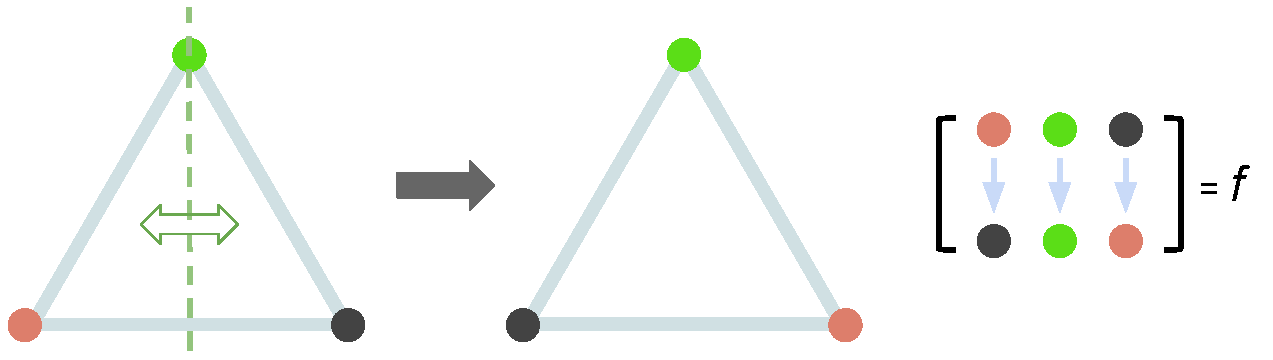
\includegraphics[width=0.8\paperwidth]{./images/Dihedral2.pdf}}
    \caption{The group action $f$ on dihedral group $D_3$ with order 6. $f$ is a horizontal flip.}
\end{figure}

We could said that the rotational symmetry group of an equilateral triangle, $C_3$, is isomorphic to
$\mathbb{Z}_3$. We can combine the horizontal reflection and rotations and form another reflection lines, 
which these reflection lines runs from one of the vertices to the center of the opposing side.

\begin{figure}[ht]
    \centering
    \makebox[\textwidth]{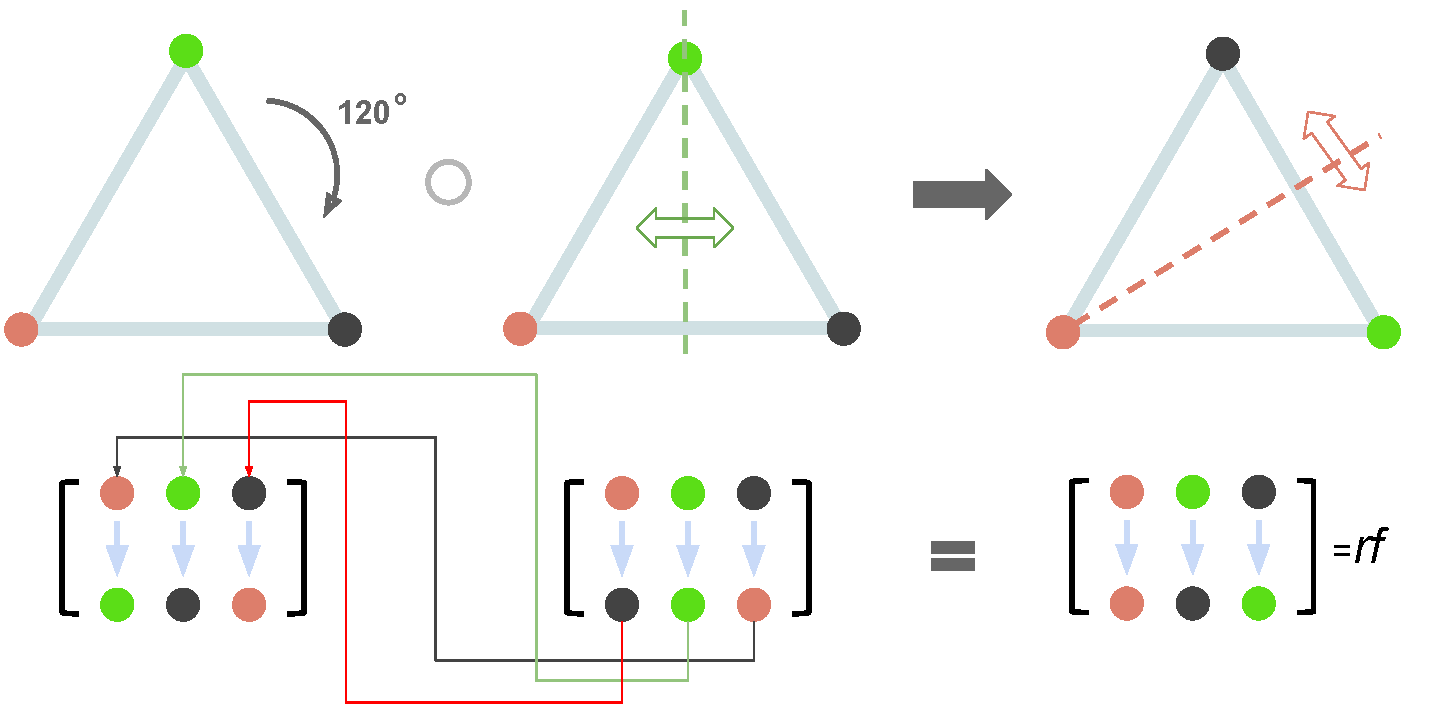
\includegraphics[width=0.8\paperwidth]{./images/Dihedral3.pdf}}
    \caption{The composition of $120\deg$ rotation with horizontal reflection form another reflection line at vertice}
\end{figure}

\begin{theorem}
    Let the $n$-degree dihedral group  
    \[
        D_n = \langle r, s \> | \> r^n = e, s^2 = e, srs = r^{-1} \rangle.
    \]
    Then 
    \begin{enumerate}
        \item $r^ks = sr^{-k}$.
        \item The order of $r^k$ is $\displaystyle \frac{n}{\gcd(n,k)}$.
    \end{enumerate}
\end{theorem}
\begin{proof}
    \begin{enumerate}
        \item Compute 
        \begin{align*}
            r^ks &= er^ks \\
            &= s^2 r^k s \\ 
            &= ssr^k s \\
            &= \fbox{$sr^{-k}$}.
        \end{align*}
        and we are done.

        \item We will first show that $r^k = e$ if and only if $n|k$. 
        
        $(\Rightarrow)$ Consider $e = r^k$, then by 
        \textit{division algorithm} we have 
        \[
            k = na+b \quad \textsf{ where } 0 \leq b < n.
        \]
        Thus 
        \[
            e = r^k = r^{na+b} = (r^n)^a\,r^b= e^ar^b = r^b.
        \]
        Since the smallest possible integer $m$ by well-ordering, such that $r^m = e$, is $n, b =0$.

        $(\Leftarrow)$ Conversely, if $n$ divide $k$, then $k = ns$ for some integer $s$. Hence 
        \[
            r^k = r^{ns} = (r^n)^s = e^s = e.
        \]

        Thus $r^k = e \Longleftrightarrow  n |k$. 
        
        Now let $b = r^k \in D_n$, since $r$ is a generator of $D_n$. We shall show that the smallest integer $m$ such that 
        $r^k = e$ is $n/k$. Let $d = \gcd(n,k)$. Consider
        \[
            e = b^m = r^{km}.
        \]
        Since this is the smallest integer $m$ such that $n|km$. Thus $\frac{n}{d}$ divide $\frac{mk}{d}$. Because $d$ 
        is the greatest common divisor of $n$ and $k$, implies $\frac{n}{d}$ and $\frac{k}{d}$ are relatively prime. Hence 
        \[
            \frac{n}{d} \bigg \vert \frac{mk}{d} \Longrightarrow \frac{n}{d} \bigg \vert m
        \]
        The smallest such $m$ is $\frac{n}{d}$. Thus 
        \[
            \ord(r^k) = \frac{n}{\gcd(n,k)}.
        \]
    \end{enumerate}
\end{proof}

\begin{example}
    Let 
    \[
        G = SL_2(\mathbb{Z}_3) = \left\{ \begin{bmatrix}
        a & b\\ c & d
        \end{bmatrix} \bigg \vert \> ad-bc \neq 0; a, b, c, d \in \mathbb{Z}_3 \right\}.
    \]
    Show that $|G| = 48$.
\end{example}
\begin{solution}
    From the first row, for all $(a,b) \in \mathbb{Z}_3 \times \mathbb{Z}_3 \setminus \{ (0,0)\}$. There are 
    $(\perm[3]{1} \times \perm[3]{1}) - 1 = 8$ possibilities.

    For the second row, for all $(c,d) \in \mathbb{Z}_3 \times \mathbb{Z}_3 \setminus (a\mathbb{Z}_3, b\mathbb{Z}_3)$.
    There are $(\perm[3]{1} \times \perm[3]{1}) - 3 = 6$ possibilities.

    Thus the order of group $G$ is the product of the number of possibilities of these two rows. $|G| = 8 \times 6 = 48$.
\end{solution}

\section{Sylow's theorem}

\begin{theorem}
    $C_5 \times C_2$ and $C_{10}$ are two isomorphism classes.
\end{theorem}
\begin{proof}
    From the \textit{Third Sylow's theorem}, the number of Sylow 5-groups divides 2 and is $1 (mod 5)$, so there is only one Sylow 5-group.
    And there is a normal subgroup $K \trianglelefteq G$ such that $|K| = 5$.
\end{proof}

\section{Automorphisms}

\begin{definition}
    An isomorphism from a group $G$ onto itself is called an automorphism.
\end{definition}

\begin{example}
    Let the 2-dimensional cartesian plane
    \[
        \mathbb{R}^2 = \{ (a,b) | a, b \in \mathbb{R} \}.
    \]
    Then
    \[
        \phi(a,b) = (b,a)
    \]
    is an automorphism of the group $\mathbb{R}^2$ under componentwise addition.
\end{example}

\begin{example}
    Compute $\text{Aut}(\mathbb{Z}_{10})$.
\end{example}
\begin{solution}
    For any $\alpha \in \text{Aut}(\mathbb{Z}_{10})$ and for any $k \in \mathbb{Z}_{10}$. We define $k \mapsto k \alpha(1)$ such that 
    \[
        1 \mapsto \alpha_1 :\quad \mathbb{Z}_{10} \to \mathbb{Z}_{10}, \quad \alpha_1(x) = x
    \]
    \[
        3 \mapsto \alpha_3 :\quad \mathbb{Z}_{10} \to \mathbb{Z}_{10}, \quad \alpha_3(x) = 3x
    \]
    \[
        7 \mapsto \alpha_7 :\quad \mathbb{Z}_{10} \to \mathbb{Z}_{10}, \quad \alpha_7(x) = 7x
    \]
    \[
        9 \mapsto \alpha_9 :\quad \mathbb{Z}_{10} \to \mathbb{Z}_{10}, \quad \alpha_9(x) = 9x
    \]

    In fact, $\text{Aut}(\mathbb{Z}_{10})$ is isomorphic to $U(10) = \{ 1, 3, 7, 9\}$.
\end{solution}

\begin{definition}[Inner automorphisms]
    Let $G$ be a group, and let $a \in G$. The function $\phi_a$ defined by 
    \[
        \phi_a(x) = axa^{-1} \quad \text{for all } x \in G
    \]
    is called the inner automorphism of $G$ included by $a$.

    When $G$ is a group, we use $\text{Aut}(G)$ to denote the set of all automorphisms of $G$ and 
    $\text{Inn}(G)$ to denote the set of all inner automorphisms of $G$.
\end{definition}

\begin{theorem}
    The set of automorphisms of a group and the set of inner automorphisms of a group are both groups under the 
    operation of function composition.
\end{theorem}
\begin{proof}
    The set of inner automorphisms of $G$ included by $a$ is 
    \[
        \text{Inn}(G) = \{ \phi_a | \phi_a \text{ is an inner automorphism}  \}.
    \]
    Then satisfied the group properties:
    \begin{enumerate}
        \item We want to show $\forall \phi_a, \phi_b \in \text{Inn}(G), \quad \phi_a \circ \phi_b \in \text{Inn}(G)$.  

        Compute $(\phi_a \circ \phi_b)(g)$ for all $g$ in $G$,
        \begin{align*}
            (\phi_a \circ \phi_b)(g) &= \phi_a (\phi_b (g))\\
            &= \phi_a(bgb^{-1}) & \text{(Defn. of inner automorphism)}\\
            &= a(bgb^{-1})a^{-1}\\
            &= (ab)g(b^{-1}\, a^{-1})\\
            &= (ab)\, g\, (ab)^{-1} & \text{(Socks-shoes property)}\\
            &= \phi_{ab}(g) \in \text{Inn}(G)
        \end{align*}
        
        Thus $\text{Inn}(G)$ is closed under function composition.

        \item Next we want to show the associativity in $\text{Inn}(G)$, that is, 
        \[
            \forall \phi_a, \phi_b, \phi_c \in \text{Inn}(G), \quad \phi_a \circ (\phi_b \circ \phi_c) = (\phi_a \circ \phi_b) \circ \phi_c 
        \]

        we compute $\phi_a \circ (\phi_b \circ \phi_c)$.
        \begin{align*}
            [\phi_a \circ (\phi_b \circ \phi_c)](g) &= a(bc)g(bc)^{-1}a^{-1}\\
            &= (ab)c g \, c^{-1}\, b^{-1}\, a^{-1}\\
            &= {\color{cyan} (ab)}{\color{red} \underline{c\, g\, c^{-1}}}\, {\color{cyan} (ab)^{-1}}\\
            &= [{\color{cyan} (\phi_a \circ \phi_b)} \circ {\color{red} \underline{\phi_c}}](g)
        \end{align*}

        \item Suppose $e$ is the identity element of $G$, then $\phi_e(g) = ege^{-1} = g \in \text{Inn}(G)$. $\phi_e$ is the 
        identity of $\text{Inn}(G)$.

        \item For all $\phi_a \in \text{Inn}(G)$, there exists $\phi_{a^{-1}} \in \text{Inn}(G)$ such that 
        \begin{align*}
            \phi_a \circ \phi_{a^{-1}} &= a(a g^{-1} a^{-1})a^{-1}\\
            &= (a\,a^{-1}) g^{-1} (a\,a^{-1})\\
            &= g^{-1}
        \end{align*}
    \end{enumerate}

    We have shown that the inner automorphisms are group. Is $\text{Inn}(G)$ a subgroup of $\text{Aut}(G)$? Of course it is. We 
    are going to use one-step subgroup test to find out.

    \textbf{One-step subgroup test}:

    \begin{enumerate}
        \item First of all, we want to show 
        \[
            \forall \phi_a, \phi_b \in \text{Inn}(G), \phi_a \circ \phi_{b^{-1}} \in \text{Inn}(G).
        \]

        we compute
        \begin{align*}
            (\phi_a \circ \phi_{b^{-1}})(g) &= \phi_a (b g^{-1}b^{-1})\\
            &= a(b g^{-1}b^{-1})a^{-1}\\
            &= (ab)g^{-1}\,(ab)^{-1}\\
            &= \phi_{(ab)^{-1}} \in \text{Inn}(G)
        \end{align*}
    \end{enumerate}
\end{proof}

\section{Cosets}

\begin{example}
    Consider $G = \mathbb{Z}_9 = \{ 0, 1, 2, \ldots, 8 \} (\text{mod} \, 9)$. We take a cyclic subgroup 
    \[H = \langle 3 \rangle = \{0, 3, 6\}\] 
    which came from $(G, +_9)$. All \textbf{left cosets} of $G$ with respect to $H$ are $\{ H, 1 +_9 H, 2 +_9 H \}$ where
    \begin{align*}
        &0 +_9 H = \{0 + 0, 0+ 3, 0 + 6\} \> (\text{mod} \, 9) = \{0, 3, 6\} = H\\
        &1H = 1 +_9 H = \{1 + 0, 1 + 3, 1 + 6\} \> (\text{mod} \, 9) = \{1, 4, 7\}\\
        &2H = 2 +_9 H = \{2 + 0, 2 + 3, 2 + 6\} \> (\text{mod} \, 9) = \{2, 5, 8\}\\
        &3H = 3 +_9 H = \{3 + 0, 3 + 3, 3 + 6\} \> (\text{mod} \, 9) = \{3, 6, 0\} = H
    \end{align*}

    As for the right cosets of $G$ with respect to $H$ are $\{ H, H +_9 1, H +_9 2 \}$. Pay attention that now the element of coset are being 
    added to right-hand side instead of from left side.

    \begin{align*}
        &0 +_9 H = \{0 + 0, 0+ 3, 0 + 6\} \> (\text{mod} \, 9) = \{0, 3, 6\} = H\\
        &H1 = H +_9 1 = \{0 + 1, 3 + 1, 6 + 1\} \> (\text{mod} \, 9) = \{1, 4, 7\}\\
        &H2 = H +_9 2 = \{0 + 2, 3 + 2, 6 + 2\} \> (\text{mod} \, 9) = \{2, 5, 8\}\\
        &H3 = H +_9 3 = \{0 + 3, 3 + 3, 6 + 3\} \> (\text{mod} \, 9) = \{3, 6, 0\} = H
    \end{align*}
\end{example}

\section{Normal subgroups, Quotient groups}

\subsection{Normal subgroups}

\begin{definition}[Normal subgroups]
    A subgroup $H$ of $(G, \cdot)$ is called a normal subgroup if for all $g \in G$ we have 
    \begin{equation}
        gH = Hg.
    \end{equation}
    We shall denote that $H$ is a subgroup of $G$ by $H < G$, and that $H$ is a normal subgroup of $G$ 
    by $H \vartriangleleft G$. 
    
    If $H$ is a normal subgroup of $G$, and the order of $H$ is equal to the order of $G$, we called $H$ the proper normal subgroup, write as $H \trianglelefteq G$. 
\end{definition}

You should be very careful here. The equality $gH = Hg$ is a set equality. They are not constants or numbers! It says that a 
right coset is equal to left a coset, it is not an equality elementwise.

\begin{example}
    Let $\mathbb{R}[x]$ denote the group of all polynomial with real coefficients under normal addition. 

    For any $f$ in $\mathbb{R}[x]$, let $f'$ denote the derivative of $f$. Then the mapping $f \to f'$ is a homomorphism from 
    $\mathbb{R}[x]$ to itself. The kernel of the derivative mapping is the set of all constant polynomials $f(x) = c$.
\end{example}

Now suppose we have a group $(G, \cdot)$, and $H$ is a normal subgroup of $G$, just said $H \vartriangleleft G$. The set $G/H$ is defined by 
\[
G/H = \{ gH \> | \> g \in H \}
\]

\begin{example}
    Show that if $H$ and $K$ are normal subgroups of a group $G$ such that $H \cap K = \{ e \}$, then 
    $hk = kh$ for all $h \in H$ and $k \in K$.
\end{example}
\begin{solution}
    We knew that $H \unlhd G$ and $K \unlhd G$, these conditions imply
    \[
        gHg^{-1} \subseteq H,\quad gKg^{-1} \subseteq K \quad \forall g \in G.
    \]
    Since $khk^{-1} \in kHk^{-1} \subseteq kHk^{-1}\subseteq H$. 
    We want to show $hk = kh$ for all $h \in H$ and $k \in K$. Compute 
    \begin{align*}
        h(kh^{-1}k^{-1}) = e &\Rightarrow hkh^{-1}k^{-1} = e\\
        &\Rightarrow hkh^{-1} = ke\\
        &\Rightarrow hkh^{-1} = khh^{-1}\\
        &\Rightarrow hk = kh.
    \end{align*}
\end{solution}

\section{Group homomorphisms}

\begin{definition}
    A group homomorphism is a map $f: (G,{\color{red} \diamond}_G) \to (H, {\color{cyan} \bullet}_H)$ that respects binary operations:
    \begin{equation}
        f(a) \> {\color{cyan} \bullet}_H \> f(b) = f(a \> {\color{red} \diamond}_G \> b) \quad \forall a, b \in G
    \end{equation}
\end{definition}

\begin{theorem}[Properties of homomorphism]
    Let $\phi$ be a homomorphism from a group $G$ to a group $G'$ and let $g$ be an element of $G$. Then
    \begin{enumerate}
        \item $\phi$ carries the identity of $G$ to the identity of $G'$.
        \item $\phi(g^n) = \left( \phi(g) \right)^n$ for all $n \in \mathbb{Z}$.
        \item If $\ord(g)$ is finite, then $\ord(\phi(g))$ divides $\ord(g)$.
        \item $ker(\phi)$ is a subgroup of $G$.
        \item $\phi(a) = \phi(b)$ if and only if $a\, ker(\phi) = b\, ker(\phi)$.
        \item If $\phi(g)= g'$, then $\phi^{-1}(g') = \{ x \in G \> | \> \phi(x) = g' \} = g\, ker(\phi)$.
    \end{enumerate}
\end{theorem}

\section{Isomorphism}
\begin{definition}[Group isomorphisms]
    An isomorphism $\phi$ from a group $G$ to a group $G'$ is a one-to-one 
mapping from $G$ onto $G'$ that preserves the group operation. That is, 
\[
    \phi(a) \> {\color{cyan} \bullet}_G \> \phi(b) = \phi(a \> {\color{red} \diamond}_{G'} \> b)
\]
for all $a,b \in G$. If there is an isomorphism from $G \to G'$, we say that $G$ and $G'$ are isomorphic 
and write as $G \cong G'$.
\end{definition}

There are four separate steps involved in proving that a group $G$ is isomorphic to another group $G'$.
\begin{enumerate}
    \item Define a candidate for the isomorphism; that is, assume that $\phi(a) = \phi(b)$ and hence prove that 
        $a=b$.
    \item Prove that $\phi$ is one-to-one; that is, assume that $\phi(a) = \phi(b)$ and hence 
    prove that $a=b$.
    \item  Prove that $\phi$ is onto; that is, for any element $g' \in G'$, find an element $g \in G$
    such that $\phi(g) = g'$.
    \item Prove that $\phi$ is operation-preserving; that is, show that 
    \[
        \phi(a) \> {\color{cyan} \bullet}_G \> \phi(b) = \phi(a \> {\color{red} \diamond}_{G'} \> b)
    \]
    for all $a, b \in G$. 
\end{enumerate}

\begin{example}
    Let $G=SL(2, \mathbb{R})$, the group of $2 \times 2$ real matrices with determinant 1. Let $M$ be 
any $2\times 2$ matrix with determinant 1. The mapping $\phi_M$ from $G \to G$ defined by
\[
    \phi_M(A) = MAM^{-1}
\]
is an isomorphism.
\end{example}
\begin{solution}
    \begin{enumerate}
        \item First we are going to show that $\phi_M$ is one-to-one; that is,
        for any $A_1, A_2 \in G$, if $\phi_M(A_1) = \phi_M(A_2)$, then $A_1 = A_2$.

        \begin{align*}
            \phi_M(A_1) = \phi_M(A_2) &\Rightarrow MA_1M^{-1} = MA_2M^{-1} \\
            &\Rightarrow {\color{red} M^{-1}} MA_1M^{-1} {\color{red} M}= {\color{red} M^{-1}} MA_2M^{-1} {\color{red} M}\\
            &\Rightarrow IA_1I = IA_2I \\
            &\Rightarrow A_1 = A_2.
        \end{align*}

        \item Show $\phi_M$ is onto. For all $A_2 \in G$, we need to find $A_1 \in G$ such that 
            \[
                \phi_M(A_1) = A_2.
            \]
            We find an equation for $A_1$,
            \begin{align*}
                \phi_M(A_1) = A_2 &\Rightarrow MA_1M^{-1} = A_2\\
                &\Rightarrow A_1 = M^{-1}A_2M
            \end{align*}
            Now we verify that $\phi_M(A_1) = A_2.$. Compute
            \begin{align*}
                \phi_M(A_1) &= \phi_M(M^{-1}A_2M)\\
                &= M\, (M^{-1}A_2M) \, M^{-1}\\
                &= IA_2I\\
                &= A_2.
            \end{align*}
        
        \item At last we are going to show $\phi_M$ is a homomorphism. That is,
            \[
                \forall A_1, A_2 \in G, \quad \phi_M(A_1\, A_2) = \phi_M(A_1)\phi_M(A_2).
            \]
            We start from LHS,
            \begin{align*}
                \phi_M(A_1\, A_2) &\Rightarrow MA_1\, A_2 M^{-1}\\
                &\Rightarrow MA_1\, {\color{red} I}\, A_2 M^{-1}\\
                &\Rightarrow MA_1\, {\color{red} (M^{-1} M)}\, A_2 M^{-1}\\
                &\Rightarrow (MA_1\,{\color{red}  M^{-1}}) ({\color{red} M} A_2\, M^{-1})\\
                &\Rightarrow \phi_M(A_1)\phi_M(A_2).
            \end{align*}
    \end{enumerate}

    Therefore $\phi_M$ is an isomorphism.
\end{solution}

\begin{example}
    The group $U(10)$ is not isomorphic to $U(12)$.
\end{example}

\begin{theorem}[Cayley's theorem]
    Every group is isomorphism to a group of permutation.
\end{theorem}
\begin{proof}
    Let $G$ be a multiplication group. From group $G$, we need to construct a permutation group $\olsi{G}$ that is 
    isomorphic to $G$.

    \subsubsection*{Step 1: construct permutation group $\olsi{G}$}

    Given $G$, for all $g \in G$. We define a map $T_g : G \to G$ such that 
    \[
        T_g(x) = gx.
    \]
    Let $\olsi{G} = \{T_g \> | \> g \in G \}$. We need to show that $\olsi{G}$ under function composition is a 
    group.

    \begin{enumerate}
        \item (Closureness) For all $T_g, T_h \in \olsi{G}$, we want to show $T_g \circ T_h \in \olsi{G}$.
            \begin{align*}
                T_g \circ T_h &= T_g \left( T_h (x)\right)\\
                &= T_g(hx)\\
                &= g(hx)\\
                &= (gh)x\\
                &= T_{gh}(x) \in \olsi{G}.
            \end{align*}
        
        \item (Associativity) For all $T_g, T_h, T_k \in \olsi{G}$, we have 
        \[
            T_g \circ (T_h \circ T_k) = T_{g(hk)} = T_{(gh)k} = (T_g \circ T_h) \circ T_k.
        \]
        The asscoiativity holds in $\olsi{G}$.

        \item (Existence of identity) For all $T_g \in \olsi{G}$, there exists an $T_{g'} \in \olsi{G}$ such that 
        \begin{align*}
            T_g \circ T_{g'} = T_g &\Rightarrow T_{gg'} = T_g\\
            &\Rightarrow gg' = g\\
            &\Rightarrow g' = 1
        \end{align*}
        so that $g'(x) = 1 \cdot x = x$.

        \item (Existence of inverse) For all $T_g \in \olsi{G}$, the inverse of $T_g$ is 
        \[
            T_{g^{-1}}(x) = g^{-1} x \quad \forall g \in G. 
        \]
    \end{enumerate}
    Therefore $\olsi{G}$ is a group under function composition. In the next step we are going to prove that 
    the mapping from $G$ to $\olsi{G}$ is an isomorphism.

    \subsubsection*{Step 2: show that $\phi: G \to \olsi{G}$ is isomorphism}

    We now define a mapping $\phi: G \to \olsi{G}$, where 
    \[
        \phi(g) = T_g(x) = gx \quad \forall g \in G.
    \]
    We perform the 3 steps to check $\phi(g)$ is an isomorphism.

    \begin{enumerate}
        \item ($\phi$ is one-to-one) For all $g, h \in G$, 
        \begin{align*}
            \phi(g) = \phi(h) &\Rightarrow T_g = T_h\\
            &\Rightarrow T_g(x) = T_h(x) \quad \forall x \in G\\
            &\Rightarrow gx = hx \quad \forall x \in G\\
            &\Rightarrow g = h.
        \end{align*}

        \item ($\phi$ is onto) For all $T_{g'} \in \olsi{G}$, we need to find an $g \in G$ such that $\phi(g) = T_{g'}$.
        \begin{align*}
            \phi(g) = T_{g'} &\Rightarrow T_g(x) = T_{g'}(x)\\
            &\Rightarrow gx = g'x\\
            &\Rightarrow g = g'.
        \end{align*}

        \item ($\phi$ is homomorphism) To show that $\phi$ is homomorphism, it is equivalent to show that  
        \[
            \phi(g \circ h) = \phi(g)\, \phi(h).
        \]
        From LHS, 
        \begin{align*}
            \phi(g \circ h) = T_{gh} &= T_{gh}(x)\\
            &= (g \circ h)x\\
            &= gx \cdot hx\\
            &= \phi(g)\, \phi(h).
        \end{align*}
    \end{enumerate}

\end{proof}

\begin{definition}[Group stabilizer]
    If $G$ is a group of permutations on the set $S$ and $s \in S$ then we define the \bred{stabilizer} 
    of $s$ to be the set 
    \[
    \stab_G(s) = \{ \phi \in G \> | \> \phi(s) = s \}.
    \]
\end{definition}

\begin{lemma}
    If $G$ is a group of permutations of the set $S$ and $s \in S$. Then $\stab_G(s)$ is a subgroup of $G$.
\end{lemma}
\begin{proof}
    Using two-step subgroup test to verify:
    \begin{enumerate}
        \item $\exists \phi: S \to S \in \stab_G(s) \> s.t. \> \phi(x) = x$. Thus $\stab_G(s) \neq \varnothing$.
        \item For all $\phi_1, \phi_2 \in \stab_G(s)$, we have 
        \[
            (\phi_1 \circ \phi_2)(s) = \phi_1 \left( \phi_2(s) \right)
            = \phi_1(s) = s \in S
        \]
        Therefore $\phi_1 \circ \phi_2 \in \stab_G(s)$.

        \item For all $\phi \in \stab_G(s)$, 
        \begin{align*}
            \phi(s) = s &\Rightarrow \phi^{-1} \left( \phi (s) \right) = \phi^{-1}(s)\\
            &\Rightarrow \phi^{-1}(s) = s \in S
        \end{align*}
        So $\phi^{-1}$ is also in $\stab_G(s)$.
    \end{enumerate}

    Therefore $\stab_G(s)$ is a subgroup of $G$.
\end{proof}

\begin{definition}[Group orbit]
    If $G$ is a group of permutations of the set $S$ and $s \in S$. We define the \bred{orbit} to be the set
    \[
        \orb_G(s) = \{ \phi(s) \> | \> \phi \in G \}.
    \]
\end{definition}

\begin{theorem}[Orbit-Stabilizer theorem]
    For any group action $\phi : G \to \text{Permutation}(S)$, and for any $s \in S$,
    \begin{equation}
        |\orb_G(s)| \cdot |\stab_G(s)| = |G|.
    \end{equation}
\end{theorem}
\begin{proof}
    We define a mapping $f: G/\stab_G(s) \to \orb_G(s)$ such that 
    \[
        f\left( \phi \stab_G(s) \right) = \phi(s).
    \]
    $f$ is a homomorphism, and we want to show $f$ is one-to-one and onto. 
    \begin{enumerate}
        \item (One-to-one) For all $\phi_1, \phi_2 \in \stab_G(s)$, we have
        \begin{align*}
            \phi_1 \stab_G(s) = \phi_2 \stab_G(s) &\Rightarrow (\phi_1^{-1} \circ \phi_2) \in \stab_G(s)\\
            &\Rightarrow (\phi_1^{-1} \circ \phi_2)(s) = s\\
            &\Rightarrow \phi^{-1} \left( \phi_2(s) \right) = s\\
            &\Rightarrow \phi_2(s) = \phi_1(s)\\
        \end{align*}

        \item (Onto) We again want to show $f$ is onto. For all $\phi \in \orb_G(s)$, we have
        \[
            f\left( \phi \stab_G(s) \right) = \phi(s).
        \]
    \end{enumerate}
    So $f$ is both one-to-one and onto. Which means 
    \begin{align*}
        |G/\stab_G(s)| = |\orb_G(s)| &\Longrightarrow \frac{|G|}{|\stab_G(s)|} = |\orb_G(s)|\\[0.5em]
        &\Longrightarrow |\orb_G(s)| \cdot |\stab_G(s)| = |G|.
    \end{align*}
\end{proof}

\newpage 
\begin{theorem}
    The group of rotations of a cube is isomorphic to $S_4$.
\end{theorem}
\begin{proof}
    We can proof it by visualizing the rigid motions of a cube rotated along the possible axes.
    \begin{figure}[ht]
        \centering
        \begin{tikzpicture}
            \begin{scope}[scale=2,y={(0.2cm,0.3cm)},x={(1cm,0cm)}, z={(0cm,1cm)}]
                \coordinate (O) at (0, 0, 0);
            
                \draw[  very thick,Bcolor, dashed ] (0,0,1)--(0,0,-1);
                \draw[  very thick,Bcolor ] (0,0,-1.4)--(0,0,-1);
                \draw[  very thick,Bcolor ] (0,0,1.4)--(0,0,1);
            
                \draw[dotted, very thick,medgrey] (1,1,-1)--(-1,1,-1)--(-1,-1,-1);
                \draw[dotted, very thick,medgrey] (-1,1,-1)--(-1,1,1);
            
                \draw[thick,opacity=0.2,fill=Ccolor]  (1,1,1)--(1,-1,1)--(-1,-1,1)--(-1,1,1)--cycle; % top
                \draw[thick,opacity=0.2,fill=Ccolor] (1,-1,1)--(1,-1,-1)--(-1,-1,-1)--(-1,-1,1)--cycle; % front
                \draw[thick,opacity=0.2,fill=Acolor] (1,1,-1)--(1,1,1)--(1,-1,1)--(1,-1,-1)--cycle;
            
              \end{scope}
              \node[inner sep = 0cm,text width=\linewidth, align=center] at (0,-5.5)   () {One of three possible axes of rotation through the centers of opposite faces.\\ Each rotation could be $0^\circ$, $90^\circ$, $180^\circ$, or $270^\circ$, for a total of $3\times 4 = 12$ rotations of this type. But three in this count are the trivial identity rotation, which we only count once, so there are really 10 unique rotations along these axes. };
        \end{tikzpicture}
    \end{figure}

    \begin{figure}[ht]
        \centering
        \begin{tikzpicture}
            \begin{scope}[scale=2,y={(0.2cm,0.3cm)},x={(1cm,0cm)}, z={(0cm,1cm)}]
                \coordinate (O) at (0, 0, 0);
            
                \draw[  very thick,Bcolor, dashed ] (-1,1,1)--(1,-1,-1);
                \draw[  very thick,Bcolor ] (1.2,-1.2,-1.2)--(1,-1,-1);
                \draw[  very thick,Bcolor ] (-1.2,1.2,1.2)--(-1,1,1);
            
            
                \draw[  dotted, very thick,medgrey ] (1,1,-1)--(-1,1,-1)--(-1,-1,-1);
                \draw[dotted, very thick ,medgrey] (-1,1,-1)--(-1,1,1);
            
                \draw[thick,opacity=0.2,fill=Ccolor]  (1,1,1)--(1,-1,1)--(-1,-1,1)--(-1,1,1)--cycle; % top
                \draw[thick,opacity=0.2,fill=Ccolor] (1,-1,1)--(1,-1,-1)--(-1,-1,-1)--(-1,-1,1)--cycle; % front
                \draw[thick,opacity=0.2,fill=Acolor] (1,1,-1)--(1,1,1)--(1,-1,1)--(1,-1,-1)--cycle;
            
              \end{scope}
              \node[inner sep = 0cm,text width=\linewidth, align=center] at (0,-5.5)   () {One of four possible axes of rotation through opposite vertices. Each could be either $120^\circ$ or $240^\circ$, so there are $4 \times 2 = 8$ rotations of this type.};
        \end{tikzpicture}
    \end{figure}

    \newpage
    \begin{figure}[ht]
        \centering
        \begin{tikzpicture}
            \begin{scope}[scale=2,y={(0.2cm,0.3cm)},x={(1cm,0cm)}, z={(0cm,1cm)}]
                \coordinate (O) at (0, 0, 0);
            
                \draw[  very thick,Bcolor, dashed ] (0,1,1)--(0,-1,-1);
                \draw[  very thick,Bcolor ] (0,-1.2,-1.2)--(0,-1,-1);
                \draw[  very thick,Bcolor ] (0,1.2,1.2)--(0,1,1);
            
                \draw[  dotted, very thick,medgrey ] (1,1,-1)--(-1,1,-1)--(-1,-1,-1);
                \draw[dotted, very thick ,medgrey] (-1,1,-1)--(-1,1,1);
            
                  \draw[thick,opacity=0.2,fill=Ccolor]  (1,1,1)--(1,-1,1)--(-1,-1,1)--(-1,1,1)--cycle; % top
                  \draw[thick,opacity=0.2,fill=Ccolor] (1,-1,1)--(1,-1,-1)--(-1,-1,-1)--(-1,-1,1)--cycle; % front
                  \draw[thick,opacity=0.2,fill=Acolor] (1,1,-1)--(1,1,1)--(1,-1,1)--(1,-1,-1)--cycle;
            
              \end{scope}
              \node[inner sep = 0cm,text width=\linewidth, align=center] at (0,-4.5)   () {One of six possible axes of rotation through the centers of opposite edges. Only a $180^\circ$ rotation around these axes would preserve the shape, so we have only 6 rotations possible.};
        \end{tikzpicture}
    \end{figure}

    There are $10 + 8 + 6 = 24$ possible ways to rotate a cube, this is equal to the order of $S_4$. The order of $S_4$ is
    \[
        |S_4| = 4! = 4 \times 3 \times 2 \times 1 = 24.
    \]
\end{proof}

\begin{theorem}[Properties of isomorphisms]
    Suppose that $\phi$ is an isomorphism from a group $G$ onto a group $G'$. Then 
    \begin{enumerate}
        \item $\phi$ carries the identity of $G$ to the identity of $G'$.
        \item For every integer $n$ and for every group element $a$ in $G$,
        \[
            \phi(a^n) = \phi(a)^n.
        \]
        \item For any elements $a$ and $b$ of $G$, $a$ and $b$ commute if and only if $\phi(a)$ and $\phi(b)$ commute.
        \item $G = \langle a \rangle$ if and only if $G' = \langle \phi(a) \rangle$.
        \item $\ord(a) = \ord(\phi(a))$ for all $a \in G$.
        \item For a fixed integer $k$ and fixed group element $b \in G$, the equation $x^k = b$ has the same number of solutions 
        in $G$ as does the equation $x^k = \phi(b) \in G'$.
        \item If $G$ is finite, then $G$ and $G'$ have exactly the same number of elements of every order.
    \end{enumerate}
\end{theorem}
\begin{proof}
    \begin{enumerate}
        \item Work with $G$, we know $e = g^n g^{-n}$, so 
        \begin{align*}
            \phi(e) = \phi(g^ng^{-n})&\Rightarrow e' = \phi(g^n) \phi(g^{-n})\\
            &\Rightarrow e' = \phi(\underbrace{g * g * \cdots * g}_{n \text{ times}})\> \phi(\underbrace{g^{-1} * g^{-1} * \cdots * g^{-1}}_{n \text{ times}})\\
            &\Rightarrow e' = \underbrace{\phi(g) * \phi(g) * \cdots * \phi(g)}_{n \text{ times}}\> \underbrace{\phi(g^{-1}) * \phi(g^{-1}) * \cdots * \phi(g^{-1})}_{n \text{ times}}\\
        \end{align*}

        \item Using the similar technique, we have 
            \[
                \phi(g^n) = \phi(\underbrace{g * g * \cdots * g}_{n \text{ times}}) = \underbrace{\phi(g) * \phi(g) * \cdots * \phi(g)}_{n \text{ times}} = \phi(g)^n.
            \]
        
        \item For all $a,b \in G$, $a$ and $b$ commute if and only if 
            \begin{align*}
                ab = ba &\Longleftrightarrow \phi(ab) = \phi(ba) \\
                &\Longleftrightarrow \phi(a) \phi(b) = \phi(b) \phi(a) \\
                &\Longleftrightarrow \phi(a) \textsf{ and } \phi(b) \textsf{ commute}\\
                &\Longleftrightarrow G' \textsf{ is abelian}.
            \end{align*}
        
        \item For all $a \in G$, 
            \begin{align*}
                G = \langle a \rangle &\Longleftrightarrow \phi(a^n) = \phi(e) \\
                &\Longleftrightarrow \phi(a^n) = e' \\
                &\Longleftrightarrow \phi(a)^n = e'\\
                &\Longleftrightarrow G' = \langle \phi(a) \rangle.
            \end{align*}
    \end{enumerate}

    (5, 6, 7) leave as tutorial.
\end{proof}

\subsection{Isomorphism theorems}

\begin{theorem}[Second Isomorphism Theorem]
    Let $K$ be a proper subgroup of $G$, and $N \triangleleft G$. Then 
    \begin{enumerate}
        \item $NK = \{ nk \> | \> n\in N, k \in K \}$ is a proper subgroup of $G$, write $NK < G$.
        \item $N \triangleleft NK$ and $K \cap N \triangleleft K$.
        \item $K/(K \cap N)$ is isomorphism to $NK/N$.
    \end{enumerate}

    \[
        \begin{tikzcd}[row sep=2.0em]
            & G \arrow[dash, "\leq"]{d} & \\
            & NK \arrow[dash]{dl} \arrow[dr, "\triangleright"] & \\
            K \arrow[dr, "\triangleright"] & & N \arrow[dash]{dl} \\
            & K \cap N & \\
        \end{tikzcd}
    \]
\end{theorem}
\begin{proof}
    \begin{enumerate}
        \item Clearly $NK \subset G$. By using two-step subgroup test. For all $nk, n'k' \in NK$
        \[
            nkn'k' = (nn')(kk') \in NK.
        \]
        and 
        \[
            nk = e \Longrightarrow nkk^{-1}n^{-1} = e \Longrightarrow (nk)^{-1} = k^{-1} n^{-1} \in NK.
        \]
        Thus $NK < G$.

        \item Clearly $N \triangleleft NK < G$, since $aN = Na$ whenever $a$ in $NK$. $N \triangleleft G$ 
        implies that the mapping $\pi: G \to G/N$ that maps $a \to Na$ is a surjective homomorphism. We 
        define $f:K \to G/N$ which $k \mapsto Nk$ whenever $k$ in $K$. Apparently $f$ is also 
        homomorphism.

        The kernel of $f$ is
        \begin{align*}
            ker\, f &= \{ k \in K \> | \> f(k) = Ne \}\\
            &= \{ k \in K \> | \> Nk = Ne \}\\
            &= \{ k \in K \> | \> k \in N \}\\
            &= K \cap N.
        \end{align*}

        Thus $K \cap N \triangleleft K$.

        \item Find the image of $f$,
        \begin{align*}
            \Ima f &= \{ Nk \in G/N \> | \> k \in K \}\\
            &= \{ Nnk \in G/N \> | \> n \in N, k \in K \}\\
            &= \{ Nnk \in G/N \> | \> nk \in NK \}\\
            &= NK/N.
        \end{align*}

        By First Isomorphism Theorem, we now have $K/(K \cap N)$ is isomorphism to $NK/N$.
    \end{enumerate}
\end{proof}

\section{Lagrange Theorem}

\begin{theorem}[Lagrange theorem]
    If $G$ is a finite group and $H$ is a subgroup of $G$, then $|H|$ divides $|G|$.
\end{theorem}
\begin{proof}
    Let $a_1H, a_2H, \ldots, a_rH$ denote the distinct left cosets and right cosets of $H$ in $G$. 
    For all $a \in G, \exists i \> s.t. \> aH =a_iH$ and $a \subseteq aH$. Thus we can say that each members in $G$ 
    belongs to the one of the cosets of $a_iH$. Since $|a_iH| = |H|$, so
    \[
        G = \bigcup^r_{k=1} a_kH \Longrightarrow |G| = \sum^{r}_{k=1} |a_kH| = \sum^{r}_{k=1} |H| = r(|H|).
    \]
    Thus $|H|$ divides $|G|$
\end{proof}

\begin{example}
    Given $G$ is a group of order 6. Find all possible subgroups of $G$.
\end{example}
\begin{solution}
    Suppose $H$ is a subgroup of $G$, $H \leq G$, and so by Lagrange's theorem we have 
    \[
        |H| \> \big \vert \> |G| = 6
    \]
    which implies $|H| \in \{1, 2, 3, 6\}$.

    If the order of $H$ is one, then $H = \langle e \rangle = \{ e \}$.

    On the other hand, when $|H| = 6$ which means $|H| = |G| = 6$ and $H = G$; that is, $H$ is trivial subgroup.

    \[
        \begin{tikzcd}[row sep=2.5em]
            & \mathbb{Z}_6 \arrow[dash, "\leq"]{dl} \arrow[dash, "\leq"]{dr} & \\
            \langle 3 \rangle \arrow[dash, "\leq"]{dr}&  & \langle 2 \rangle \arrow[dash, "\leq"]{dl}\\
            & \{ 0 \} &\\
        \end{tikzcd}
    \]
\end{solution}

\begin{theorem}
    If $G$ is a group of order $p$, where $p$ is a prime. Then $G$ is cyclic.
\end{theorem}
\begin{proof}
    Suppose $H$ is a subgroup of $G$ and we apply Lagrange's theorem, which we have 
    \[
        |H| \> \big \vert \> |G| = p.
    \]
    Assume $H \neq \{ e \}$ and the order of $H$ is greater than one, implies $|H| = p$ and so $|G| = |H| = p$.

    Hence, since $H \neq \{ e \}$, then there exists $a \neq e$ and $a \in H$. So using $a$ to generate we obtained
    \[
        H = G = \langle a \rangle
    \]
    implies that $H$ and $G$ are both cyclic.
\end{proof}

\section{External Direct Product}

\begin{definition}[External direct product]
    Given groups $(G, *)$ and $(H, +)$, the external direct product of 
    $G, H$ written as $G \oplus H$, is the set of all ordered pairs $(g,h)$ for which the 
    the binary operation on $G \oplus H$ is defined component-wise:
    \[
        (g_1, h_1) \oplus (g_2, h_2) = (g_1 * g_2, h_1 + h_2).
    \]
\end{definition}

The resulting algebraic object satisfies the axioms for a group.

\begin{example}
    Find $U(8) \oplus U(10)$.
\end{example}
\begin{solution}
    \begin{center}
        \begin{tabular}{c|cccc}
            & 1 & 3 & 7 & 9\\
        \end{tabular}
    \end{center}
\end{solution}

\section{Internal Direct Product}

\begin{definition}
    Let $(G, *) be a group and let $
\end{definition}

\section{Finite Abelian groups}

\begin{theorem}[Fundamental theorem of Finite Abelian groups]
    Every finite Abelian group is a direct product of cyclic groups of 
prime-power order. Moreover, the number of terms in the product and the orders of 
the cyclic groups are uniquely determined by the group.

Since a cyclic group of order n is isomorphic to $\mathbb{Z}_n$. Then every finite Abelian group 
$G$ is isomorphic to a group of the form
\[
    \mathbb{Z}_{p_1^{n_1}} \oplus \mathbb{Z}_{p_2^{n_2}} \oplus \cdots \oplus \mathbb{Z}_{p_k^{n_k}}
\]
where $i$'s are not necessarily distinct primes and the prime powers $p_1^{n_1}, p_2^{n_2}, \ldots, p_k^{n_k}$ are uniquely 
determined by $G$.
\end{theorem}

 
Look at groups whose orders have the form $p_k$, where $p$ is prime and $j \leq 4$. There is 
one group of order $p_k$ for each set of positive integers whose sum is $k$ (such a set is 
called a partition of $k$); that is, if $k$ can be written as $k = n_1 + n_2 + \cdots + n_t$, where 
each $n_i$ is a positive integer, then $\mathbb{Z}_{p_1^{n_1}} \oplus \mathbb{Z}_{p_2^{n_2}} \oplus \cdots \oplus \mathbb{Z}_{p_t^{n_t}}
$ is an Abelian group 
of order $p^k$.

\begin{center}
    \begin{tabular}{c|c|c}
        Order of $G$ & Partitions of $k$ & Possible direct products of $G$\\[0.3em]
        \hline
        $p$ & $1$ & $\mathbb{Z}_p$\\[0.3em]
        \hline
        $p^2$ & $2$ & $\mathbb{Z}_{p^2}$\\[0.3em]
        & $1+1$ & $\mathbb{Z}_p \oplus \mathbb{Z}_p$\\[0.3em]
        \hline
        $p^3$ & $3$ & $\mathbb{Z}_{p^3}$\\[0.3em]
        & $1+2$ & $\mathbb{Z}_p \oplus \mathbb{Z}_{p^2}$\\[0.3em]
        & $1+1+1$ & $\mathbb{Z}_p \oplus \mathbb{Z}_p \oplus \mathbb{Z}_p$\\[0.3em]
        \hline
        $p^4$ & $4$ & $\mathbb{Z}_{p^4}$\\[0.3em]
        & $1+3$ & $\mathbb{Z}_p \oplus \mathbb{Z}_{p^3}$\\[0.3em]
        & $2+2$ & $\mathbb{Z}_{p^2} \oplus \mathbb{Z}_{p^2}$\\[0.3em]
        & $1+1+2$ & $\mathbb{Z}_p \oplus \mathbb{Z}_p \oplus \mathbb{Z}_{p^2}$\\[0.3em]
        & $1+1+1+1$ & $\mathbb{Z}_p \oplus \mathbb{Z}_p \oplus \mathbb{Z}_p \oplus \mathbb{Z}_p$\\[0.3em]
        \hline
    \end{tabular}
\end{center}

\subsection{Greedy algorithm for an Abelian group of order $p^n$}

Here are the procedure to find all the possible abelian group of order $p^n$. Note that $p$ is prime.

\begin{enumerate}
    \item Compute the orders of the elements of the group $G$.
    \item Select an $a_1$ of maximum order and define $G_1 = \langle a_1 \rangle$. Set $i = 1$.
    \item If $|G| = |G_i|$, stop. Otherwise, replace $i$ by $i + 1$.
    \item Select an element $a_i$ of maximum order $p^k$ such that 
    \[
        p^k \leq |G|/|G_{i-1}|
    \]
    and none of $a_i, a_i^{p}, a_i^{p^2}, \ldots, a_i^{p^{k-1}}$ is in $G_{i-1}$, and define $G_i = G_{i-1} \times \langle a_i \rangle$.
    \item Return to step 3.
\end{enumerate}

In the general case where $|G| = p_1^{n_1}\, p_2^{n_2}\, \ldots p_k^{n_k}$, we simply use the algorithm to build 
up a direct product of order $p_1^{n_1}$, then another of order $p_2^{n_2}$, and so on.  The direct 
product of all these pieces is the desired factorization of $G$.

\begin{algorithm}[ht]
    \caption{Greedy algorithm for an Abelian group of order $p^n$}
    \tcp{Main body of greedy algorithm for finding Abelian group of order $p^k$.}
    \Function{Main\_greedy\_algorithm($G$: FiniteGroup) $\to$ Product of CyclicGroups}{
        \boxit{codegreen}{16.5}
        $\olsi{a} \gets $ \var{find\_element\_with\_max\_order$(G)$}\;
        \tcp{Generated subgroup with first element $\olsi{a}_1$ from $\olsi{a}$.}
        $H \gets \langle \olsi{a}_1 \rangle$\;
        $i \gets 1$\;

        \boxit{codeyellow}{11.5}
        \While(\Comment{Greedy search for all cyclic groups}){$|H| \neq |G|$}{

            $\var{max\_cyclic\_order} = |G| / |H|$\; 
            $\langle a_i \rangle = [\>]$\;
            
            \boxit{codered}{6}
            \While(){$p^k \leq \var{max\_cyclic\_order}$}{
                \eIf (\Comment{Check if $\olsi{a}^{p^{k-1}}_i$ already in previous $H$}){$\olsi{a}^{p^{k-1}}_i \notin H$}{
                    $\langle a_i \rangle$.push($\olsi{a}^{p^{k-1}}_i$)\;
                }{
                    \Continue
                }
                $k \gets k+1$\;
            }
            $H \gets H \times \langle a_i \rangle$\;
            $i \gets i + 1$\;
        }
        \Return{$H$}\;
    }

    \tcp{Compute the orders for all elements in group $G$.}
    \Function{compute\_orders($G$: FiniteGroup) $\to orders$}{
        \boxit{codegreen}{9}
        $orders = [\>]$\;
            \For(\Comment{elements in X}){$a_i \in G$} {
                \boxitt{codered}{6.5}
                \eIf () {$a_i == $ identity$(G)$}{
                    return 1   \Comment{The order of identity element is one.}
                }{
                    $j \gets 1$\;
                    \While{$a^j_i \neq e$}{ 
                        $j \gets j + 1$   \Comment{Find the order of each element.}
                    }
                    $orders$.push($j$)
                }
            }
        \Return{$orders$}\;
    }

    \tcp{Filter out $a_i$ with maximum order, return a list of tuple $(a_i, |\langle a_i \rangle|)$.}
    \Function{find\_element\_with\_max\_order($G$: FiniteGroup) $\to$ Array<tuple(element, order)>}{
        \boxit{codegreen}{2}
        $orders \gets \var{max\_cyclic\_order}(G)$\;
        \Return{zip($G$, $orders$).filter($(\_, o) \to o == $ Max($orders$))}\;
    }
\end{algorithm}

\begin{example}
    Let $G =\{1, 8, 12, 14, 18, 21, 31, 34, 38, 44, 47, 51, 52, 57, 64 \}$ under multiplication modulo $65$. 
    Show that $G$ is isomorphic to $\mathbb{Z}_4 \oplus \mathbb{Z}_4$.
\end{example}
\begin{solution}
    Since $G$ has order 16, we have 
    \begin{align*}
        G &\cong \mathbb{Z}_{16}\\
        &\cong \mathbb{Z}_{2^4} & \text{take } p=2, k = 4\\
        &\cong \mathbb{Z}_{2} \oplus \mathbb{Z}_{2^3} & \text{Partitions of } k = 1 + 3\\
        &\cong \mathbb{Z}_{2^2} \oplus \mathbb{Z}_{2^2} & \text{Partitions of } k = 2 + 2\\
        &\cong \mathbb{Z}_{4} \oplus \mathbb{Z}_{4}
    \end{align*}
\end{solution}

\begin{example}
    Let $G =\{1, 8, 17, 19, 26, 28, 37, 44, 46, 53, 62, 64, 71, 73, 82, 89,\\ 91, 98, 107,
    109, 116, 118, 127, 134 \}$ under multiplication modulo $135$. 
    Show that $G$ is isomorphic to $\mathbb{Z}_{12} \oplus \mathbb{Z}_2$.
\end{example}
\begin{solution}
    Since $G$ has order 24, and the prime factorization of $24 = 3 \cdot 2^3$. We have 
    \begin{align*}
        G &\cong \mathbb{Z}_{24}\\
        &\cong \mathbb{Z}_{3} \oplus \mathbb{Z}_{2^3}\\
        &\cong \mathbb{Z}_{3} \oplus \mathbb{Z}_{2^2} \oplus \mathbb{Z}_2\\
        &\cong \mathbb{Z}_{3} \oplus \mathbb{Z}_{4} \oplus \mathbb{Z}_2\\
        &\cong \mathbb{Z}_{3 \times 4} \oplus \mathbb{Z}_2 & \text{Since } \mathbb{Z}_p \oplus \mathbb{Z}_q \cong \mathbb{Z}_{pq} \\
        &\cong \mathbb{Z}_{12} \oplus \mathbb{Z}_2
    \end{align*}
\end{solution}

\section*{Tutorials}

\begin{mdframed}
    \vspace{-0.25cm}
    \hspace{-0.25cm}
    \begin{Exercise}
        Prove whether the following group $G$ together with operation $*$ is a group.
        \begin{enumerate}
            \item Let $*$ defined on $G = \mathbb{R}$ by letting $a * b = ab \quad \forall a, b \in \mathbb{R}$.
            \item Let $*$ defined on $G = 2\mathbb{Z}$ by letting $a * b = a + b \quad \forall a, b \in 2\mathbb{Z}$.
            \item Let $*$ defined on $G = \mathbb{R}^*$ by letting $a * b = \sqrt{ab} \quad \forall a, b \in \mathbb{R}^*$.
            \item Let $*$ defined on $G = \mathbb{Z}$ by letting $a * b = \max \{a,b\} \quad \forall a, b \in \mathbb{Z}$.
        \end{enumerate}
    \end{Exercise}

    \vspace{0.752cm}
    \begin{Exercise}
        Determine whether the given set of matrices under the specified operation, matrix addition or multiplication, is a group.
        \begin{enumerate}
            \item All $2 \times 2$ diagonal matrices under matrix addition.
            \item All $2 \times 2$ diagonal matrices under matrix multiplication.
            \item All $2 \times 2$ diagonal matrices with no zero diagonal entry under under matrix multiplication.
            \item All $2 \times 2$ diagonal matrices with all diagonal entries either $1$ or $-1$ under matrix multiplication.
            \item All $2 \times 2$ upper-triangular matrices under matrix multiplication.
            \item All $2 \times 2$ upper-triangular matrices under matrix addition.
            \item All $2 \times 2$ upper-triangular matrices with determinant $1$ under matrix multiplication.
            \item All $2 \times 2$ upper-triangular matrices with determinant either $1$ or $-1$ under matrix multiplication.
        \end{enumerate}
    \end{Exercise}

    \vspace{0.752cm}
    \begin{Exercise}
        Prove whether 
        \[
            G = \biggl\{ \begin{bmatrix}
            a & b \\ c & d
            \end{bmatrix} \bigg \vert \> ad - bc \neq 0,\> a,b,c,d \in \mathbb{Z} \biggr\}
        \]
        is a group under matrix multiplication.
    \end{Exercise}

    \vspace{0.752cm}
    \begin{Exercise}
        Prove whether 
        \[
            G = \biggl\{ \begin{bmatrix}
            a & b \\ 0 & d
            \end{bmatrix} \bigg \vert \> ad \neq 0,\> a,b,d \in \mathbb{Z} \biggr\}
        \]
        is a non-abelian group under matrix multiplication.
    \end{Exercise}

    \vspace{0.752cm}
    \begin{Exercise}
        Prove whether 
        \[
            G = \biggl\{ \begin{bmatrix}
            a & b \\ 0 & a^{-1}
            \end{bmatrix} \bigg \vert \> a \neq 0,\> a,b \in \mathbb{Z} \biggr\}
        \]
        is an abelian group under matrix multiplication.
    \end{Exercise}

    \vspace{0.752cm}
    \begin{Exercise}
        Let $(G, *)$ be a group and suppose that 
        \[
            a * b * c = e \quad \forall a,b,c \in G.
        \]

        Show that $b * c * a = e$.
    \end{Exercise}

    \vspace{0.752cm}
    \begin{Exercise}
        Show that if every element of the group $G$ is its own inverse, then $G$ is abelian.
    \end{Exercise}

    \vspace{0.752cm}
    \begin{Exercise}
        Show that every group with identity $e$ and $x \cdot x = x$ for all $x \in G$ is abelian.
    \end{Exercise}

    \vspace{0.752cm}
    \begin{Exercise}
        Show that if $G$ is a finite group with identity $e$ and with even number of elements, then there is an 
        $a \neq e$ in $G$ such that $a * a = e$.
    \end{Exercise}

    \vspace{0.752cm}
    \begin{Exercise}
        Suppose $G$ is a group such that 
        \[
            (ab)^2 = a^2\, b^2 \quad \forall a, b \in G.
        \]

        Show that $G$ is abelian.
    \end{Exercise}

    \vspace{0.752cm}
    \begin{Exercise}
        Find the order of the following cyclic groups.
        \begin{enumerate}
            \item The subgroup of $U(6)$ generated by $\displaystyle \cos \biggl( \frac{2\pi}{3}\biggr) + i \sin \biggl( \frac{2\pi}{3}\biggr)$.
            \item The subgroup of $U(5)$ generated by $\displaystyle \cos \biggl( \frac{4\pi}{3}\biggr) + i \sin \biggl( \frac{4\pi}{3}\biggr)$.
            \item The subgroup of $\mathbb{Z}/4\mathbb{Z} \times \mathbb{Z}/6\mathbb{Z}$ generated by $(1,5)$.
        \end{enumerate}
    \end{Exercise}

    \vspace{0.752cm}
    \begin{Exercise}
        Let $a$ and $b$ be elements of a group $G$. Show that if $ab$ has finite order $n$, then $ba$ also has order $n$.
    \end{Exercise}

    \vspace{0.752cm}
    \begin{Exercise}
        Show that a group with no proper nontrivial subgroup is cyclic. 
    \end{Exercise}

    \vspace{0.752cm}
    \begin{Exercise}
        Let $G$ be a nonabelian group with center $Z(G).$ Show that there exists an abelian subgroup $H$ of 
        $G$ such that $Z(G) \subset H$ but $Z(G) \neq H$. 
    \end{Exercise}

    \vspace{0.752cm}
    \begin{Exercise}
        Find all subgroups of the following groups and draw the subgroups diagram for the subgroups. 
        Hence, list all orders of the subgroups of the given groups.
        \begin{enumerate}
            \item $\mathbb{Z}_{36}$
            \item $\mathbb{Z}_{60}$
        \end{enumerate} 
    \end{Exercise}

    \vspace{0.752cm}
    \begin{Exercise}
        \begin{enumerate}
            \item Find all the proper nontrivial subgroups of $\mathbb{Z}_2 \times \mathbb{Z}_2 \times \mathbb{Z}_2$.
            \item Find all the subgroups of $\mathbb{Z}_2 \times \mathbb{Z}_4$ of order 4. 
        \end{enumerate}
    \end{Exercise}

    \vspace{0.752cm}
    \begin{Exercise}
        \begin{enumerate}
            \item Are the groups $\mathbb{Z}_2 \times \mathbb{Z}_{12}$ and $\mathbb{Z}_4 \times \mathbb{Z}_{6}$ isomorphic?
            \item Are the groups $\mathbb{Z}_8 \times \mathbb{Z}_{10} \times \mathbb{Z}_{24}$ and $\mathbb{Z}_4 \times \mathbb{Z}_{12} \times \mathbb{Z}_{40}$ isomorphic?
        \end{enumerate}
    \end{Exercise}

    \vspace{0.752cm}
    \begin{Exercise}
        Find the conjugacy classes of dihedral group $D_8$. 
    \end{Exercise}

    \vspace{0.752cm}
    \begin{Exercise}
        Show that a group that has only finite number of subgroups must be a finite group.
    \end{Exercise}

    \vspace{0.752cm}
    \begin{Exercise}
        Find all cosets of the subgroup $4\mathbb{Z}$ of $\mathbb{Z}$.
    \end{Exercise}

    \vspace{0.752cm}
    \begin{Exercise}
        Compute the quotient group $\mathbb{Z}_{12}/ \langle 2 \rangle$.
    \end{Exercise}

    \vspace{0.752cm}
    \begin{Exercise}
        Show that if $H$ is a subgroup of index 2 in a finte group $G$, then every left coset of $H$ is also a 
        right coset of $H$.
    \end{Exercise}

    \vspace{0.752cm}
    \begin{Exercise}
        Let $\phi: G \to G$ be a mapping defined by 
                \[
                    \phi(x) = x^3 \quad \forall x \in G
                \]
                where $G = \mathbb{R} \setminus \{ 0 \}$ is a group defined under usual multiplication. Show that 
                $\phi$ is a homomorphism, and hence find $ker(\phi)$.
    \end{Exercise}

    \vspace{0.752cm}
    \begin{Exercise}
        Let $\phi: G \to G$ be a mapping defined by 
                \[
                    \phi(x) = 5^x \quad \forall x \in G
                \]
                where $G = \mathbb{R} \setminus \{ 0 \}$ is a group defined under usual multiplication. Show that 
                $\phi$ is a homomorphism, and hence find $ker(\phi)$.
    \end{Exercise}

    \vspace{0.752cm}
    \begin{Exercise}
        Let $\phi: G \to G$ be a mapping defined by 
                \[
                    \phi(x) = 7x \quad \forall x \in G
                \]
                where $G = \mathbb{Z}$ is a group defined under usual addition. Show that 
                $\phi$ is a homomorphism, and hence find $ker(\phi)$.
    \end{Exercise}

    \vspace{0.752cm}
    \begin{Exercise}
        Let $G$ be a group and $g$ an element in $G$. Consider the mapping $\phi:G \to G$ defined as 
        $\phi(x) = gxg^{-1}$. Show that $\phi$ is an isomorphism.
    \end{Exercise}

    \vspace{0.752cm}
    \begin{Exercise}
        Find $ker(\phi)$ for map $\phi : \mathbb{Z}_{10} \to \mathbb{Z}_{20}$ such that 
        $\phi(1) = 8$.
    \end{Exercise}

    \vspace{0.752cm}
    \begin{Exercise}
        Find $ker(\phi)$ for map $\phi : \mathbb{Z} \times \mathbb{Z} \to \mathbb{Z} \times \mathbb{Z}$ such that 
        $\phi(1,0) = (2, -3)$ and $\phi(0,1) = (-1, 5)$.
    \end{Exercise}

    \vspace{0.752cm}
    \begin{Exercise}
        Let $\phi: G \to H$ be a group homorphism. Show that $\phi(G)$ is abelian if and only if
        \[
            xyx^{-1}y^{-1} \in ker(\phi) \quad \forall x, y \in G.
        \]
    \end{Exercise}

    \vspace{0.752cm}
    \begin{Exercise}
        Consider $A$ the set of affine maps of $\mathbb{R}$, that is 
        \[
            A = \{ f : x \mapsto ax + b, a \in \mathbb{R}^*, b \in \mathbb{R} \}
        \]
        \begin{enumerate}
            \item Show that $A$ is a group with respect to the composition of map.
            \item Let 
                \[
                    N = \{ g: x \mapsto x + b, b \in \mathbb{R} \}
                \]

                Show that $N \vartriangleleft A$.
            \item Show that the quotient group $A/N$ is isomorphic to $\mathbb{R}^*$.
        \end{enumerate}
    \end{Exercise}

    \vspace{0.752cm}
    \begin{Exercise}
        Let $G = S_4$ and let 
        \[
            H = \{ e, (1\> 2)(3 \> 4), (1\> 3)(2\> 4), (1\> 4)(2 \> 3)\}
        \]
        \begin{enumerate}
            \item Show that $H$ is a normal subgroup of $G$.
            \item Let $\overline{H} = \{ \sigma \in S_4 \> | \> \sigma(4) = 4 \}$. Define $\sigma : \overline{H} \to \text{Aut}(H)$
                by $\sigma(\tau) = \sigma \tau \sigma^{-1}$ for $\sigma \in \overline{H}$. Prove that 
                \[
                    \overline{H} \ltimes_\sigma H \cong S_4.
                \]
        \end{enumerate}
    \end{Exercise}

    \vspace{0.752cm}
    \begin{Exercise}
        Find (up to isomorphism) all abelian groups of order 45.
    \end{Exercise}

    \vspace{0.752cm}
    \begin{Exercise}
        Show that any group of order $p^2$ is abelian.
    \end{Exercise}

    \vspace{0.752cm}
    \begin{Exercise}
        Let $G$ be a group of order $pq$, where $p$ and $q$ are prime numbers. Show that every proper subgroup of $G$
        is cyclic.
    \end{Exercise}


    \vspace{0.752cm}
    \begin{Exercise}
        If $H, K \leq G$, show that $H \cap K \leq G$.
    \end{Exercise}

    \vspace{0.752cm}
    \begin{Exercise}
        If $N \vartriangleleft G$ and $H \leq G$, show that $NH \leq G$.
    \end{Exercise}

    \vspace{0.752cm}
    \begin{Exercise}
        If $N_1, N_2 \vartriangleleft G$, show that $N_1 \cap N_2 \vartriangleleft G$.
    \end{Exercise}


    \vspace{0.752cm}
    \begin{Exercise}
        If $N \vartriangleleft G$ and $H \leq G$, show that $H \cap N \vartriangleleft G$.
    \end{Exercise}
\end{mdframed}